\section{Bildverarbeitung}
\subsection{Maße zur Beurteilung von Bildern}


\subsubsection{Histogramme}
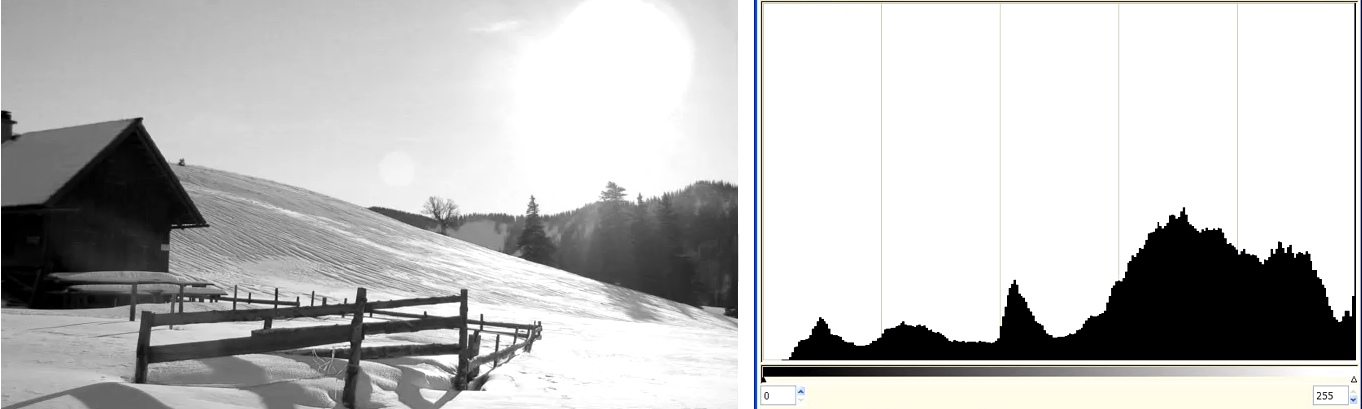
\includegraphics[height=150px]{Histogramm1.png}

Mit Histogrammen stellen wir die Häufigkeitsverteilung von Werten von Pixeln in einem Bild dar. Da wir mit 8 Bit Wertebereicht [0, 255] arbeiten, gibt es 256 Werte denen eine absolute Häufigkeit im Bereich [0, n] zugeordnet wird, wobei n die Anzahl der Pixel des Bildes ist.\\
Aus diesen Histogrammen kann man Informationen über das Bild extrahieren. Beispielsweise kann man im oberen Beispiel anhand des Histogramms sehen, dass der Großteil der Pixel einen hohen Wert hat, also das Bild eher hell ist. Des Weiteren können wir folgende Dinge erkennen:
\begin{itemize}
    \item \textbf{Belichtungsfehler:}\\
          Belichtungsfehler kann man daran erkennen, dass in einem Bild das eine Ende des Wertebereichs ungenutzt bleibt, am anderen Ende aber Häufungen auftreten (wie im oberen Beispiel)
    \item \textbf{Kontrast:}\\
          Der Kontrast bezeichnet die Differenz zwischen dem minimalen und maximalen genutzten Grauwert. Ein maximaler Kontrast nutzt den vollen Wertebereich. Das bedeutet bei 8 bit Bildern, dass es jeweils mindestens ein Pixel mit den Werten 0 und 255 im Bild geben muss. ein kleiner Kontrast entsteht, wenn alle genutzten Werte nah beieinander liegen, bis hin zum minimalen Kontrast, bei dem jedes Pixel den gleichen Wert hat.
    \item \textbf{Dynamik:}\\
          Die Dynamik beschreibt wie hoch der Anteil der genutzten Werte im Bereich zwischen dem minimalen und maximalen genutzten Wert liegt. Das bedeutet, dass eine minimale Dynamik entsteht, wenn es nur Pixel mit den Werten 0 und 255 gibt. Dann ist nämlich der genutzte Wertebereich maximal, nämlich [0, 255], und die Anzahl der genutzten Werte dieses Bereichs minimal, nämlich 2. Eine maximale Dynamik entsteht dann, wenn alle Werte zwischen dem höchsten und niedrigsten genutzten Wert genutzt werden. Das obere Bild zeigt z.B. eine maximale Dynamik, da im Wertebereich [20, 255] alle Werte mindestens 1 mal vorkommen und es keine Werte außerhalb dieses Bereichs gibt, die genutzt werden.
\end{itemize}

\subsubsection{Entropie}
Die Entropie einer Nachricht (hier eines Bildes) ist ihr mittlerer Informationsgehalt.
Es gilt: Je mehr Pixel es mit dem gleichen Wert gibt, desto geringer ist der Informationsgehalt dieser Pixel. Das bedeutet, dass die Entropie zunimmt, wenn sich die Verteilung der Grauwerte eines Bilds einer Gleichverteilung mit vollem Kontrast annähert. Auf die mathematische Berechnung wollen wir an dieser Stelle verzichten.

\subsection{Punktoperationen \& lineare Transformationen}
\label{sec:Punktoperationen}
Punktoperationen bezeichnen eine Art von Transformationen bei denen auf jedes Pixel eines Bildes eine Funktion angewendet wird, um das Pixel des Abbilds zu erzeugen, die \textbf{unabhängig von den anderen Pixeln ist}. Das bedeutet, dass die Eingangsvariable der Wert genau eines Pixel ist und die Ausgangsgröße genau der Wert des gleichen Pixels im Abbild. Die Operation wird dann für alle Pixel des Bildes durchgeführt.\\
Die Punktoperationen, die wir betrachten, sind \textbf{lineare Operationen} deshalb nennt man sie auch \textbf{lineare Grauwerttransformationen}. Das bedeutet, dass die Zuordnung eines Wertes eines Pixels im Originalbild zum Pixel im Abbild durch eine lineare Funktion beschrieben wird. Diese Funktion ordnet jedem Wert des farblichen Wertebereichs [0, 255] wieder einen Wert genau dieses Bereichs zu. Die Funktionsgraphen in denen wir das Aufzeichnen nennen wir auch gg\'-Diagramme. Im Grunde ist es eine einfache lineare Funktion. Jedoch können wir auf der x-Achse eine konkrete Verteilung (also ein Histogramm) einzeichnen, und dann die Verteilung dort auf der y-Achse einzeichnen, wo die Säulen der x-Achse auf den Funktionsgraphen treffen würden. So erkennen wir beispielsweise, dass ein Histogramm bei einer Steigung $0 < m < 1$ gestaucht wird (also der Kontrast verringert wird) und für $m > 1$ das Histogramm gestreckt wird (also der Kontrast vergrößert wird). Im unteren Beispiel ist unsere Funktion $g' = g$, die also das Bild auf sich selbst abbildet.\\

Dabei ist unbedingt zu beachten, dass der Funktionsgraph eine ganz normale lineare Funktion ist, die auch ohne das Histogramm dargestellt werden kann. Die Funktion ordnet jedem Farbwert (x-Wert) einen neuen Ergebniswert (y-Wert) zu. Das Histogramm ist nur eine Veranschaulichung der konkreten Anwendung für mehrere Punkte. Wir setzen also den Grauwert jedes Pixels einzeln in die Funktion ein, um seinen Ergebnispixel zu erhalten. Das Histogramm zeigt uns für ein konkretes Bild wie oft welcher x-Wert eingesetzt werden wird.

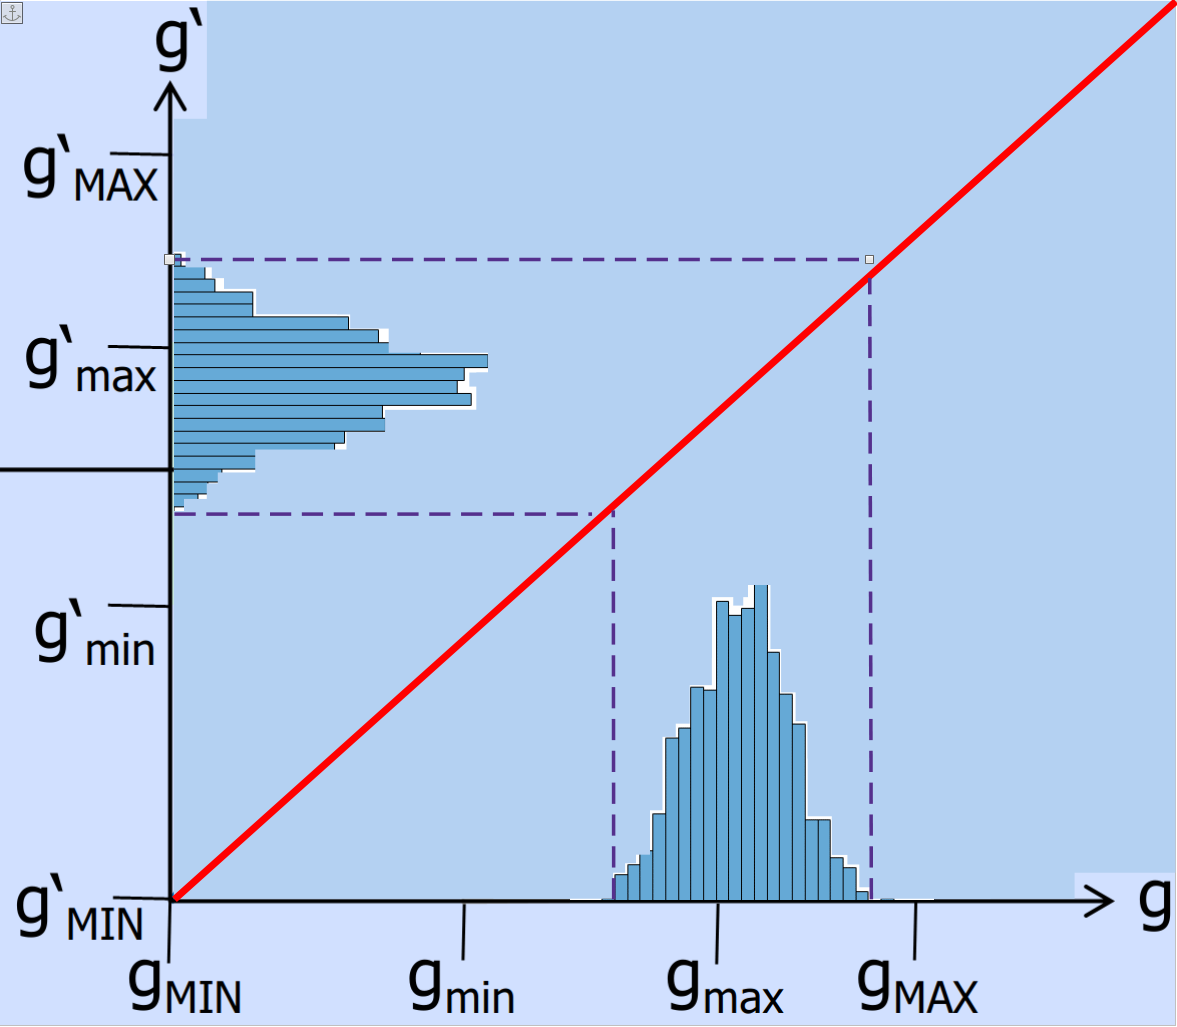
\includegraphics[height=200px]{ggstrichDiagramm.png}

Bei der Wahl der Funktion für die lineare Grauwerttransformation müssen wir darauf achten, dass wir den Wertebereich der Funktion einschränken. Der Definitionsbereich und der Wertebereich müssen meist beide innerhalb unseres Bereichs von Farbwerten, also [0, 255], liegen, damit das Ergebnis wieder ein gültiges Bild ist. Um dies umzusetzen können wir Mathematisch beispielsweise eine min bzw. max Funktion benutzen. Programmiertechnisch gibt es natürlich noch viele andere Wege dieses recht einfache problem zu lösen.\\
Es kann jedoch auch Anwendungsfälle geben, in denen der Definitionsbereich oder Wertebereich nicht [0, 255] sein müssen. Bei den \hyperref[sec:difference-operator]{Differenzoperatoren} werden wir beispielsweise sehen, dass wir die lineare Grauwerttransformation anwenden, um Ergebniswerte wieder in den gültigen Bereich zu bewegen. In diesem Fall können die Eingangswerte z.B. auch negativ sein.
Im folgenden sollen einige Punktoperationen beispielhaft gezeigt werden:\\

\subsubsection{Addition}

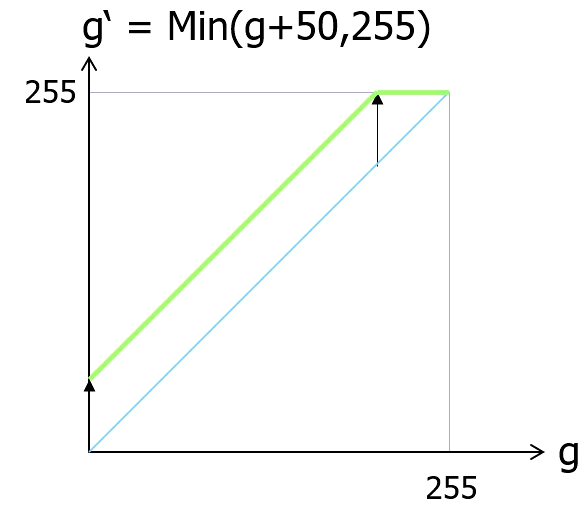
\includegraphics[height=150px]{PunktoperationAddition.png}

Bei dieser Addition wird auf jeden Pixelwert 50 addiert. Das interessante daran ist, dass der Wertebereich [0, 49] des Ergebnisbildes auf jeden Fall ungenutzt bleibt. Außerdem werden alle Säulen des Histogramms von [205, 255] auf den Wert 255 abgebildet. Dadurch entsteht, falls der Bereich [205, 255] überhaupt im Originalbild genutzt wurde, eine erhöhte Häufigkeit für den Pixelwert 255 im Ergebnisbild. Ansonsten sind im Ergebnishistogramm bloß alle Werte um 50 nach rechts verschoben. Logisch gesehen beschreibt die Addition mit einem positiven Wert eine gleichmäßige Aufhellung des Bildes.

\subsubsection{Biniarisierung}
\label{sec:biniarisierung}

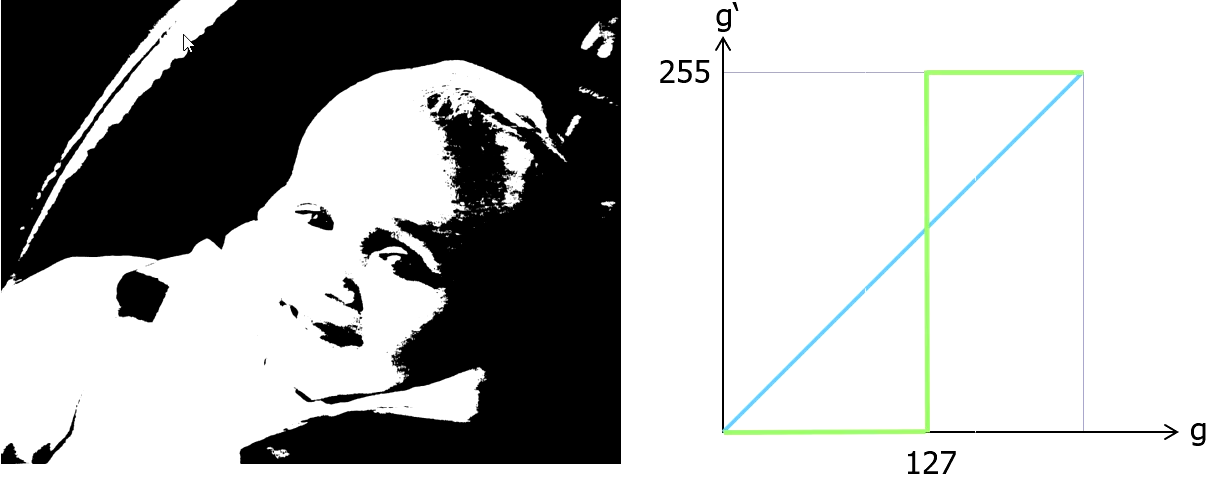
\includegraphics[height=150px]{PunktoperationBiniarisierung.png}

Die Biniarisierung ist eine lineare Grauwerttransformation, bei der die Mächtigkeit des Wertebereichs 2 ist $|W| = 2$. Dabei kann gewählt werden bei welchem Schwellwert der Umbruch vom einen Wert auf den anderen erfolgt (im Beispiel 127) und auf welche 2 Werte abgebildet wird (im Beispiel auf die Werte 0 und 255).

\subsubsection{Äquidensitenbilder}

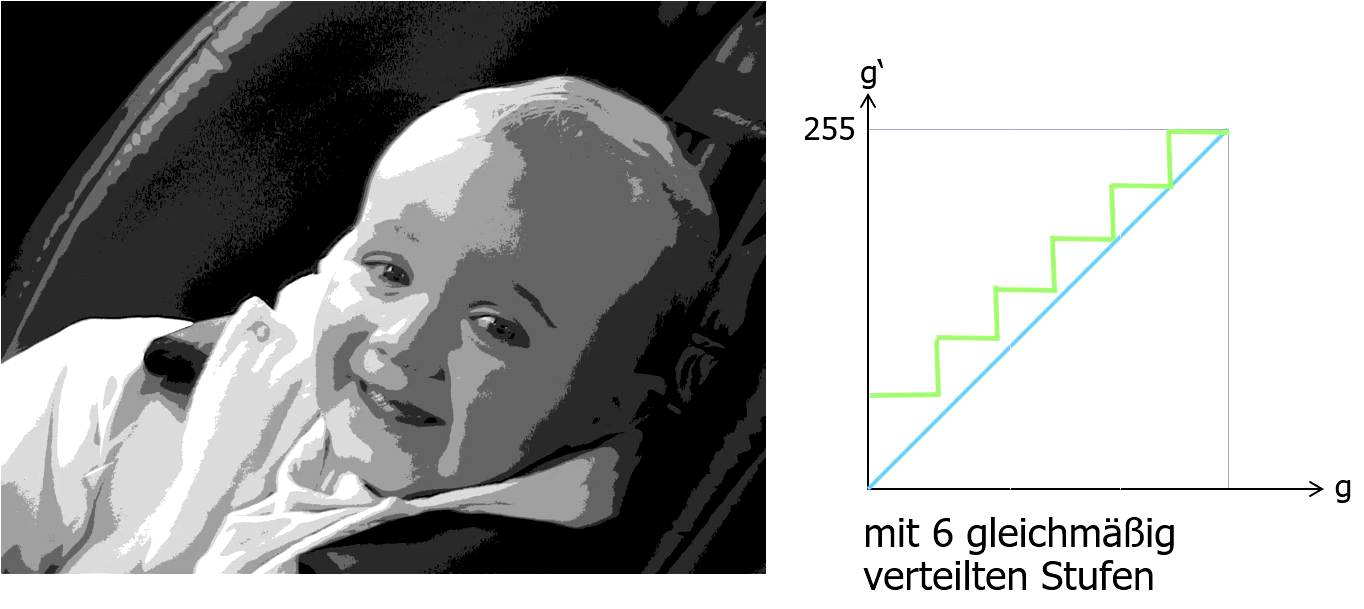
\includegraphics[height=150px]{PunktoperationAequidensitenbild.png}

Bei einem Äquidensitenbild wird der Wertebereich auf einige (im Beispiel 6) gleich weit voneinander entfernte Werte eingeschränkt. Das entspricht einer Biniarisierung mit einem Wertebereich mit mehr als 2 Elementen. Je mehr verschiedene Farbwerte genutzt werden, desto weniger auffallend ist diese lineare Grauwerttransformation. Diese Transformation findet Anwendung beim Drucken. Denn hier stehen eventuell nicht alle Farbwerte zur Verfügung. Deshalb müssen dann einige benachbarte Farbwerte auf die selbe Druckerfarbe abgebildet werden.

\subsubsection{Kontrastveränderung}

\includegraphics[height=150px]{KontrasterhöhungVorher.png} \hspace{200px}
\includegraphics[height=150px]{KontrasterhöhungNachher.png}

\includegraphics[height=100px]{KontrasterhöhungHistogrammVorher.png}
\hspace{150px}
\includegraphics[height=100px]{KontrasterhöhungHistogrammNachher.png}

Die Kontrastveränderung können wir zum Beispiel anwenden, um den Kontrast zu erhöhen, wenn ein Bild keinen vollen Kontrast hat, es also links oder rechts im Histogramm gibt, die nicht genutzt werden. Um das Bild auf einen vollen Kontrast zu transformieren muss die in schwarz eingezeichnete Grauwerttransformation durchgeführt werden. Es wird eine Gerade von $P_1=(g_{min}, g'_{MIN})$ bis $P_2=(g_{max}, g'_{MAX})$gezogen werden. Dabei sind $g_{min}$ und $g_{max}$ die minimalen und maximalen genutzten Grauwerte im Originalwert und $g'_{MIN}$ und  $g'_{MAX}$ die Grenzen des Wertebereichs im Ergebnisbild. der Bereich von $g'_{MIN}$ bis $g'_{MAX}$ bestimmt also welche Spanne von Werten das Ergebnisbild einnimmt und ist somit bei einer Erhöhung auf vollen Kontrast $g'_{MIN}=0$ und $g'_{MAX}=255$.\\
Man sieht, dass auf diese Weise Lücken im Histogramm entstehen, die Dynamik also abnimmt, die Entropie bleibt gleich, da es immernoch genau gleich viele unterschiedliche Pixelwerte mit der gleichen Verteilung gibt, nur haben sich die konkreten Werte geändert.\\

Beachte unbedingt die \hyperref[sec:Punktoperationen]{Einführung in die Punktoperationen}, um den Graphen richtig zu verstehen.

\subsection{Lokale Bildoperationen - Faltungsoperatoren}

\subsubsection{Faltungsmatrizen /-operatoren und deren Berechnung}
\label{sec:faltungsoperatoren}

\textbf{N4-Nachbarschaft}\\

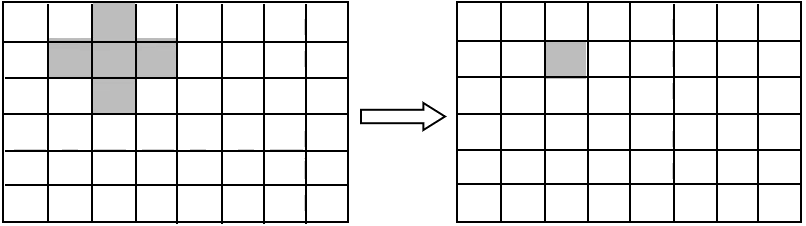
\includegraphics[height=70px]{N4Nachbarschaft.png}

\textbf{N8-Nachbarschaft}\\

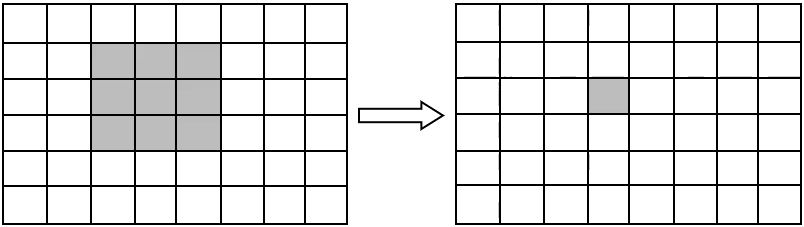
\includegraphics[height=70px]{N8Nachbarschaft.png}

Lokale Bildoperationen sind Transformationen, bei denen für die Berechnung eines Pixels mehrere, nämlich sinnvoller Weise benachbarte, Pixel betrachtet werden. Bei den Nachbarschaftsbeziehung unterscheiden wir zwischen N4- und N8-Nachbarschaft, in welchen einem Pixel, das in der Mitte liegt, jeweils 4 oder 8 Nachbarn zugeordnet werden.\\
Haben wir uns für eine Nachbarschaftsform entschieden, dann müssen wir für jedes Pixel der ''Schablone'', auch Faltungsmatrix genannt, eine Gewichtung definieren. Bei der Berechnung eines Pixelwertes wird jeder Wert der Schablone mit dem Wert des jeweiligen Pixels multipliziert und dann alle so entstandenen Werte addiert. Zur Berechnung aller Pixel des Ergebnisbildes wird nun die Berechnung mit der Faltungsmatrix für jeden Pixel durchgeführt, also so, dass jedes Pixel des Originalbildes einmal in der Mitte der Faltunsmatrix liegt. Eine Ausnahme ist der äußere Rand des Originalbildes, für den es keine äußeren Nachbarn gibt. Deshalb wird der Rand weggelassen und das Ergebnisbild in beide Richtungen 2 Pixel kleiner.\\
In vielen Fällen ist der Wertebereich nicht mehr identisch mit dem Definitionsbereich $D \neq W$. In diesen Fällen müssen die Werte durch eine \hyperref[sec:Punktoperationen]{Lineare Transformation} wieder in den gültigen Bereich versetzt werden. Somit können wir lokale Operationen für Schwarz weiß Bilder anwenden. Wenn wir ein Farbbild haben führen wir die Berechnungen einfach für jeden Farbchannel durch. Im folgenden sehen wir die Berechnungsformel für eine N8-Faltungsmatrix:

$e(i, j) = \sum_{l=0}^{2} \sum_{k=0}^{2} [g(i-1+k, j-1+l) \cdot f(k, l)] $

Hierbei ist $g(a, b)$ der Wert des Pixels der Faltungsmatrix in der Zeil $a$ und der Spalte $b$. $f(a, b)$ ist der Wert des Pixels im Originalbild in der Zeile $a$ und der Spalte $b$. $e(i, j)$ ist der Wert des Pixels in der Zeile i und der Spalte b.\\
Die Summenzeichen sorgen dafür, dass wie mit einer verschachtelten for-Schleife über alle 9 Pixel der Faltungsmatrix iteriert wird.\\

Nun werden wir einige Beispiele für Faltungmatrizen sehen.

\subsubsection{Identität}

$
    I
    =
    \begin{pmatrix}
        0 & 0 & 0 \\
        0 & 1 & 0 \\
        0 & 0 & 0 \\
    \end{pmatrix}
$

Die Identität ist die Faltungsmatrix bei der nur der Wert des inneren Pixels beachtet wird. Dadurch bildet sie das Originalbild auf sich selbst ab und ist identisch mit der Punktoperation $g'(i,j) = g(i,j)$

\subsubsection{Glättungsfilter / Box-Filter / Mittelwertoperator}
\label{sec:mean-operator}

$
    A
    =
    \begin{pmatrix}
        1 & 1 & 1 \\
        1 & 1 & 1 \\
        1 & 1 & 1 \\
    \end{pmatrix}
$

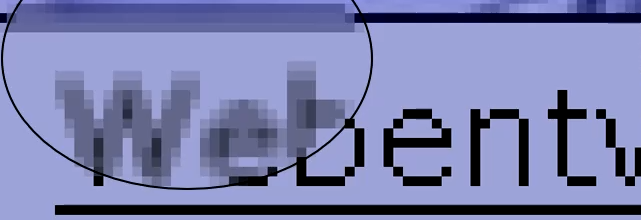
\includegraphics[height=50px]{Glaettungsfilter.png}

Bei diesem einfachen Glättungsfilter wird jedes Pixel der Faltungsmatrix gleich stark Gewichtet. Dabei entsteht im Bild eine Unschärfe oder Glättung, weil die benachbarten Pixel verschwimmen. Allerdings entstehen um Kanten herum sogenannte \textbf{ringing artifacts}. Das sind Pixel, die um die Kanten herum liegen und den gleichen Farbwert wie die Kante haben. Somit wird es schwer die Schrift zu lesen.

\subsubsection{Gauß-Filter}

$
    A
    =
    \begin{pmatrix}
        1 & 2 & 1 \\
        2 & 4 & 2 \\
        1 & 2 & 1 \\
    \end{pmatrix}
$

\includegraphics[height=50px]{GaußFilter.png}

Der Gauß-Filter ist eine Glättungsfunktion, bei der die Gewichtung der inneren Pixel höher ist. Dadurch wird das Bild zwar geglättet, aber markante Punkte bleiben erkenntbar. Im Gegensatz zum normalen Glättungsfilter können wir hier die Schrift des damit erzeugten Bildes noch besser lesbar und die linien sind besser erkennbar.

\subsubsection{Differenzoperator \& Verständnis für die Ableitung}
\label{sec:difference-operator}

$
    A
    =
    \begin{pmatrix}
        0 & 0  & 0 \\
        0 & -1 & 1 \\
        0 & 0  & 0 \\
    \end{pmatrix}
    ,
    B
    =
    \begin{pmatrix}
        0  & 0 & 0 \\
        -1 & 1 & 0 \\
        0  & 0 & 0 \\
    \end{pmatrix}
    ,
    C
    =
    \begin{pmatrix}
        0 & -1 & 0 \\
        0 & 1  & 0 \\
        0 & 0  & 0 \\
    \end{pmatrix}
    ,
    D
    =
    \begin{pmatrix}
        0 & 0  & 0 \\
        0 & -2 & 1 \\
        0 & 1  & 0 \\
    \end{pmatrix}
$

\vspace{5px}

Der Differenzoperator hat seinen Namen davon, dass er differenziert also die Ableitung bildet. Dazu muss man sich nebeneinanderliegende Pixel zunächst als Funktion vorstellen, wobei jeder Pixelwert ein Funktionswert ist. Die Ableitung kann berechnet werden, indem für jeden Pixel die Steigung berechnet wird. Da wir es mit einem diskreten Definitionsbereich zu tun haben ist die Berechnung der Steigung in einem Punkt sehr einfach. Wir subtrahieren die Differenz der Funktionswerte (Pixelwerte) von benachbarten x-Werten (Pixeln) und Teilen durch deren Differenz der x-Werte. Da die Pixel benachbart sind ist ihre Differenz auf der x-Achse 1, wodurch die Division entfällt. Mit dieser Vorstellung sollte klar sein, dass $A$ und $B$ das identische Ergebnis, nämlich die Zeilenweise Ableitung bilden. $C$ bildet die spaltenweise Ableitung. $D$ bildet die Ableitung in Zeilen- und Spaltenrichtung, was einer hinternanderausführung von $A$ und $C$ entspricht. Da die Anwendung der Transformation auf eine Summe herausläuft können wir die Summe auch in der Matrix $D$ zusammenfassen.\\

Die Differenzoperatoren haben die Eigenschaft, dass Ergebnispixel stark positive Werte annehmen, wenn im Bild eine Kante von dunkel nach hell sichtbar war, stark negative Werte annehmen, wenn eine Kante von hell nach dunkel war und 0 sind, wenn benachbarte Pixel den gleichen Farbwert hatten. Somit wird klar, dass starke Kontraste hervorgehoben werden und schwache Kontraste weiter gedämpft werden.\\

Der Wertebereich von Differenzoperatoren ist grundlegend ungültig. Für $A$ ist er z.B. [-255, 255]. Um den Wertebereich wieder in den gültigen bereich zu transformieren wird eine \hyperref[sec:Punktoperationen]{lineare Transformation} durchgeführt, die zunächst den Wertebereich auf die selbe Mächtigkeit bringt, d.h. $|W|=256$ und dann auf [0, 255] verschiebt. Im Falle von $A$ wäre das dann die lineare Transformationsfunktion $f(x)=0.5x \cdot 128$

\subsubsection{Prewitt-Operator}

$
    A
    =
    \begin{pmatrix}
        -1 & 0 & 1 \\
        -1 & 0 & 1 \\
        -1 & 0 & 1 \\
    \end{pmatrix}
    ,
    B
    =
    \begin{pmatrix}
        -1 & -1 & -1 \\
        0  & 0  & 0  \\
        1  & 1  & 1  \\
    \end{pmatrix}
$

\vspace{5px}

Der Prewitt-Operator ist im Grunde nur eine Abwandlung des Differenzoperators. Hier wird sozusagen der Sichbereich erweitert.

\subsubsection{Sobel-Operator}
\label{sec:sobel-operator}

$
    A
    =
    \begin{pmatrix}
        -1 & 0 & 1 \\
        -2 & 0 & 2 \\
        -1 & 0 & 1 \\
    \end{pmatrix}
    ,
    B
    =
    \begin{pmatrix}
        -1 & -2 & -1 \\
        0  & 0  & 0  \\
        1  & 2  & 1  \\
    \end{pmatrix}
$

Der Sobel-Operator ist wiederum eine Variation des Prewitt-Operators.

\subsubsection{Laplace-Operator}

$
    A
    =
    \begin{pmatrix}
        0 & 1  & 1 \\
        1 & -4 & 1 \\
        0 & 1  & 0 \\
    \end{pmatrix}
$

\vspace{5px}

Der Laplace-Operator bildet die 2. Ableitung in Zeilen- und in Spaltenrichtung. Wir sehen also, dass der Laplace-Operator entsteht, wenn wir von den \hyperref[sec:difference-operator]{Differenzoperatoren} 2 spaltenweise Operatoren und 2 zeilenweise Operatoren addieren. Wir könnten das gleiche Ergebnis auch mit einer nicht-punktsymmetrischen Matrix erzielen, indem wir z.B. die \hyperref[sec:difference-operator]{Matrix $D$} 2 mal anwenden, also alle Werte elementweise mit 2 multiplizieren.

\subsubsection{Kantenhervorhebung bzw. Schärfungsfilter}
Die Kantenhervorhebung nimmt einen Kantendetektor (meist Laplace) und gibt dem inneren Pixel eine beliebige Wertigkeit $n$. Somit lässt sich das aktuelle Pixel stärker gewichten. Auf diese Weise kann ein Filterergebnis mit dem Originalbild vermischt werden. Je größer $n$ gewählt wird, desto mehr fällt das Originalbild ins Gewicht.\\
Beispiel für den kantenhervorhebenden Laplace-Filter:


$
    A
    =
    \begin{pmatrix}
        0  & -1    & -1 \\
        -1 & n + 4 & -1 \\
        0  & -1    & 0  \\
    \end{pmatrix}
$


\includegraphics[height=100px]{ausgangsbild.png}

\includegraphics[height=100px]{kantenhervohebung.png}

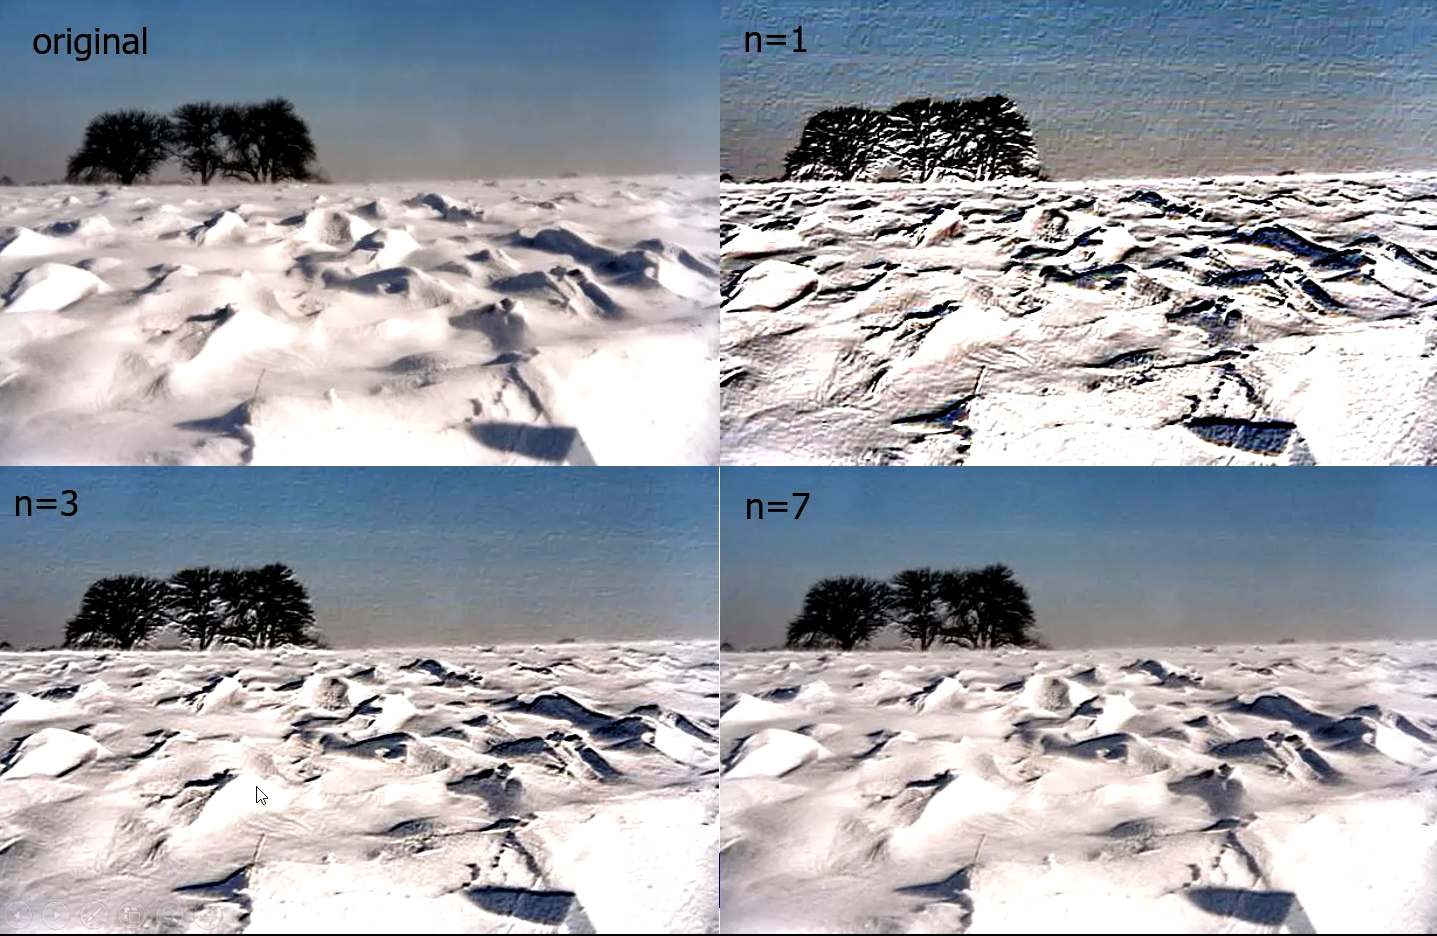
\includegraphics[width=400px]{relief-laplace-filter.png}

\subsubsection{Relief-Filter}

$
    A
    =
    \begin{pmatrix}
        -2 & -1 & 0 \\
        -1 & 1  & 1 \\
        0  & 1  & 2 \\
    \end{pmatrix}
$


\includegraphics[height=100px]{ausgangsbild.png}
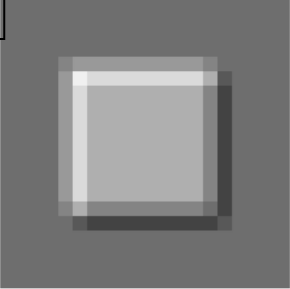
\includegraphics[height=100px]{relif-filter.png}

\subsection{Lokale Bildoperatoren - Rangfolgeoperatoren}

\subsubsection{Rangfolgeoperatoren und deren Berechnung}

Rangfolgeoperatoren sind grundlegend ähnlich wie Faltungsoperatoren. Daher empfiehlt es sich das Kapitel \hyperref[sec:faltungsoperatoren]{Faltungsoperatoren} als Einstieg zu lesen. Bei Rangfolgeoperatoren wird nämlich ebenfalls zunächst eine Nachbarschaftsbeziehung gewählt und die entstandene Matrix pixelweise über das Bild bewegt, um den Wert für das mittlere Pixel zu berechnen. Die Berechnung des Ergebnispixels erfolgt aber nicht über eine kumulierte Multiplikation, sonder über eine Auswahl genau eines Wertes aus den eingehenden Pixelwerten:\\

Wir betrachten das Beispiel einer N8-Nachbarschaft, also einer 3x3-Matrix.
\begin{enumerate}
    \item Bei der Berechnung eines Pixel werden zunächst die Werte der Eingangspixel der größe nach geordnet.
    \item Dann wird einer der Werte nach einer gewissen Vorschrift ausgewählt. Konkrete Vorschriften folgen im nächsten \hyperref[sec:types-of-ranking-operators]{Teilkapitel}.
\end{enumerate}

\subsubsection{Arten von Rangfolgeoperatoren}
\label{sec:types-of-ranking-operators}

Wir wollen hier 3 verschiedene Rangfolgeoperatoren kennenlernen und beispielhaft ihre Auswirkungen betrachten:

\textbf{Medianoperator}\\

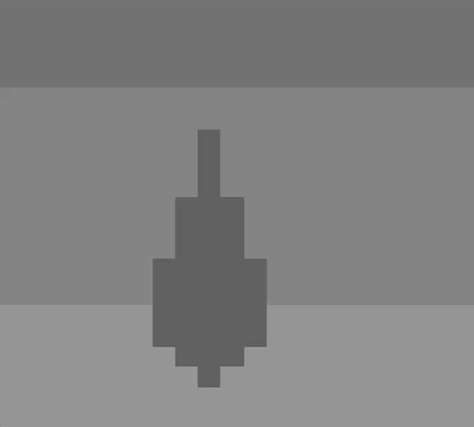
\includegraphics[height=150px]{medianoperator1.png}
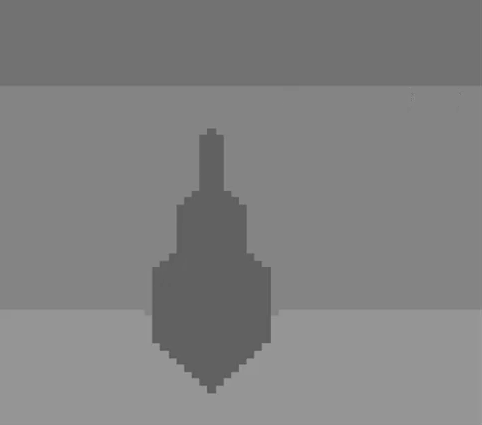
\includegraphics[height=150px]{medianoperator2.png}

Beim Medianoperator wird der Median unserer Eingangswerte, also der mittlere Wert der Rangfolge, übernommen. Das Ergebnis ist, dass Ecken abgerundet werden, aber im Gegensatz zum \hyperref[sec:mean-operator]{Mittelwertoperator} keine verschwommenen Kanten entstehen, da keine Werte gemischt werden.\\


\textbf{Erosion}\\

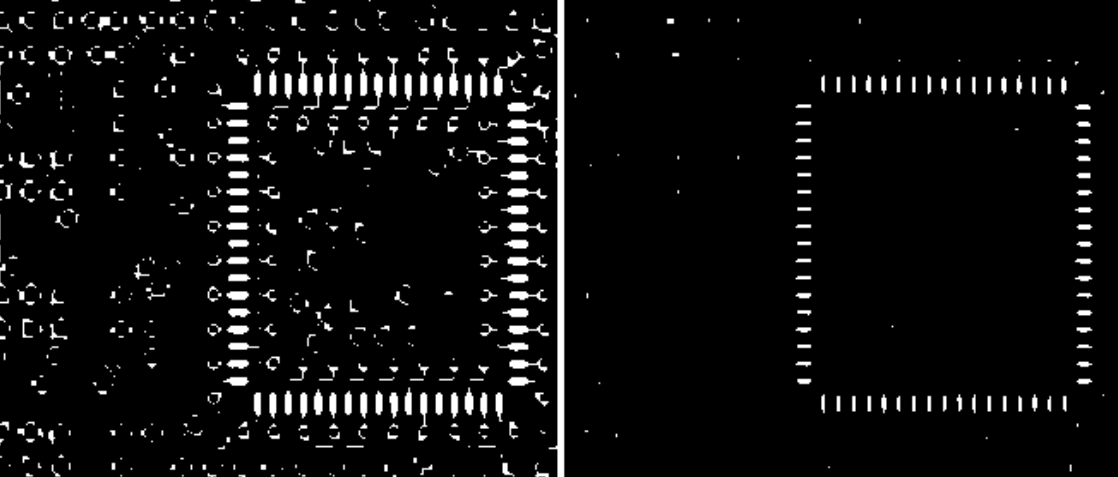
\includegraphics[height=150px]{erosion.png}

Bei der Erosion wird der dunkelste, also geringste Wert der Rangfolge übernommen. Das bedeutet, dass helle Teile an ihren Kanten, also dort wo sie auf dunklere Teile treffen, kleiner werden und dunkle Teile größer. Falls ein helles Objekt kleiner als die Rangfolgenmatrix ist verschwindet es komplett, da für jeden Punkt mindestens ein umliegender Punkt heller als das Objekt ist.\\

\textbf{Dilatation}\\

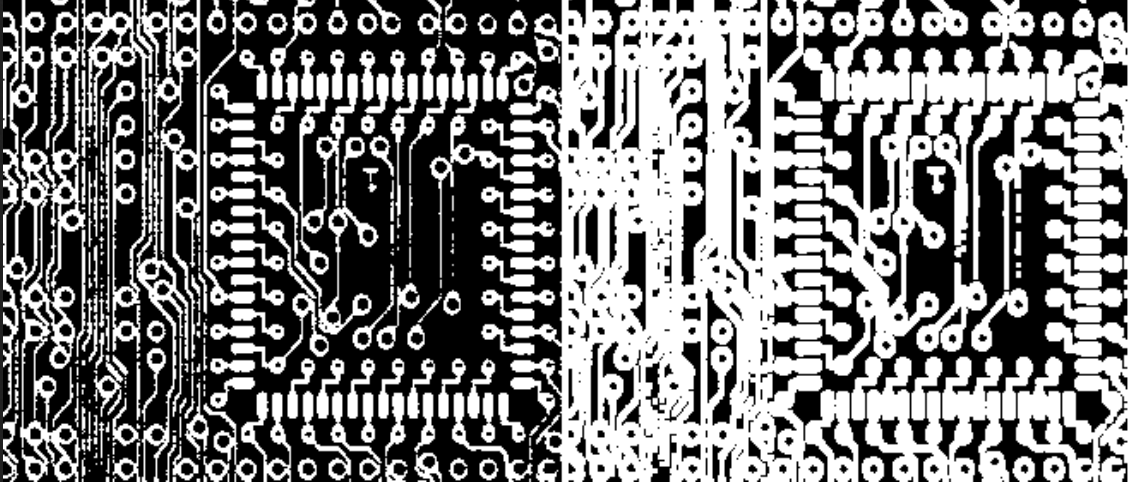
\includegraphics[height=150px]{diliatation.png}

Hier wird der hellste, also höchste Wert übernommen, dementsprechend das logische Gegenstück zur Erosion.

\subsubsection{Anwendung und Kombination von Rangfolgeoperatoren}

Die Anwendung von Rangfolgeoperatoren kann gut benutzt werden, um die Komplexität eines Bildes so stark zu vermindern, dass nur noch die relevanten Teile vorhanden sind. Solche Bilder können dann als Input für KIs dienen, welche die Bilder dann auswerten können. Wir benennen die folgenden Kombinationen:
\begin{itemize}
    \item \textbf{Opening:} erst Erosion dann Dilatation
    \item \textbf{Closing:} erst Dilatation dann Erosion
\end{itemize}

Wir wollen an einem Beispiel nun zeigen, wie wir ein Bild verarbeiten können. Dazu wenden wir folgende Schritte an:
\begin{itemize}
    \item Biniarisierung mit Schwellwert 225
    \item Closing\\
          \begin{itemize}
              \item Dilatation
              \item Erosion
          \end{itemize}
    \item Opening\\
          \begin{itemize}
              \item Erosion
              \item Dilatation
          \end{itemize}
\end{itemize}

\vspace{5px}

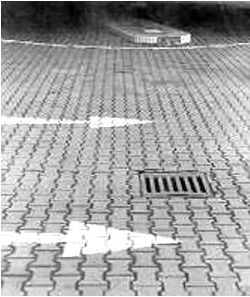
\includegraphics[height=100px]{pfeil1.png}
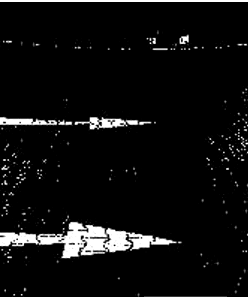
\includegraphics[height=100px]{pfeil2.png}
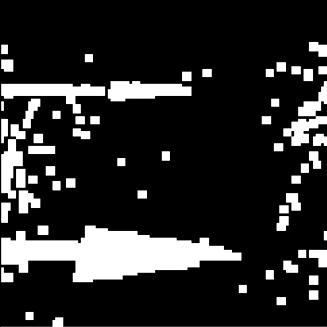
\includegraphics[height=100px]{pfeil3.png}
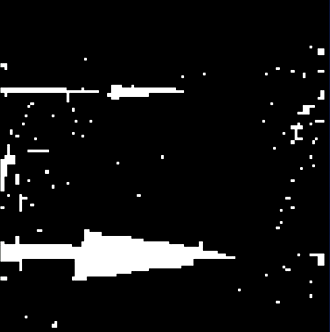
\includegraphics[height=100px]{pfeil4.png}
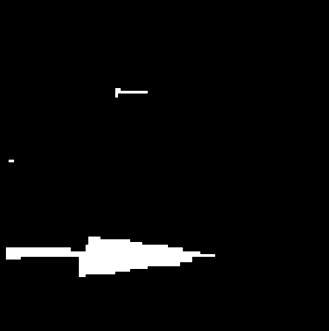
\includegraphics[height=100px]{pfeil5.png}

Damit Objekte gleich groß bleiben müssen genau so viele Erosionen wie Dilatationen durchgeführt werden. Dies gilt unter der vorraussetzungen, dass die Objekte vor jeder Iteration noch mindestens so groß wie die Rangfolgenmatrix sind, damit sie nicht vollständig verschwinden.

\subsection{Algorithmen}

\subsubsection{Canny-Edge-Detector}
\label{sec:canny-edge-detector}

Der Canny-Edge-Detector ist ein Algorithmus zur Kantenerkennung, der aus mehreren Faltungsoperationen besteht und dazu führen soll, dass das Ergebnisbild im Idealfall nur noch die Kanten des Eingangsbild enthält. Den Algorithmus kann man in 5 Schritte unterteilen, die wir hier einmal vorgestellt und erklärt werden sollen:

\subsubsection*{(i) Konvertierung zum Graubild}

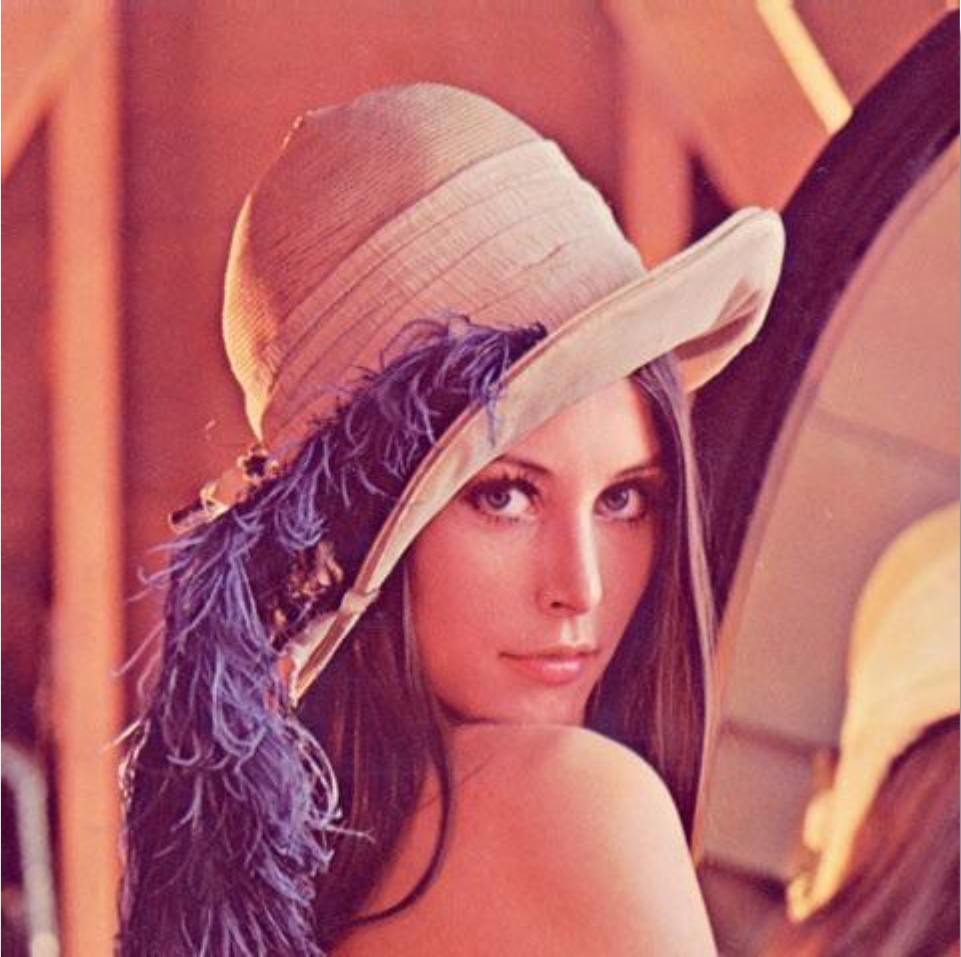
\includegraphics[height=200px]{canny-1.png}
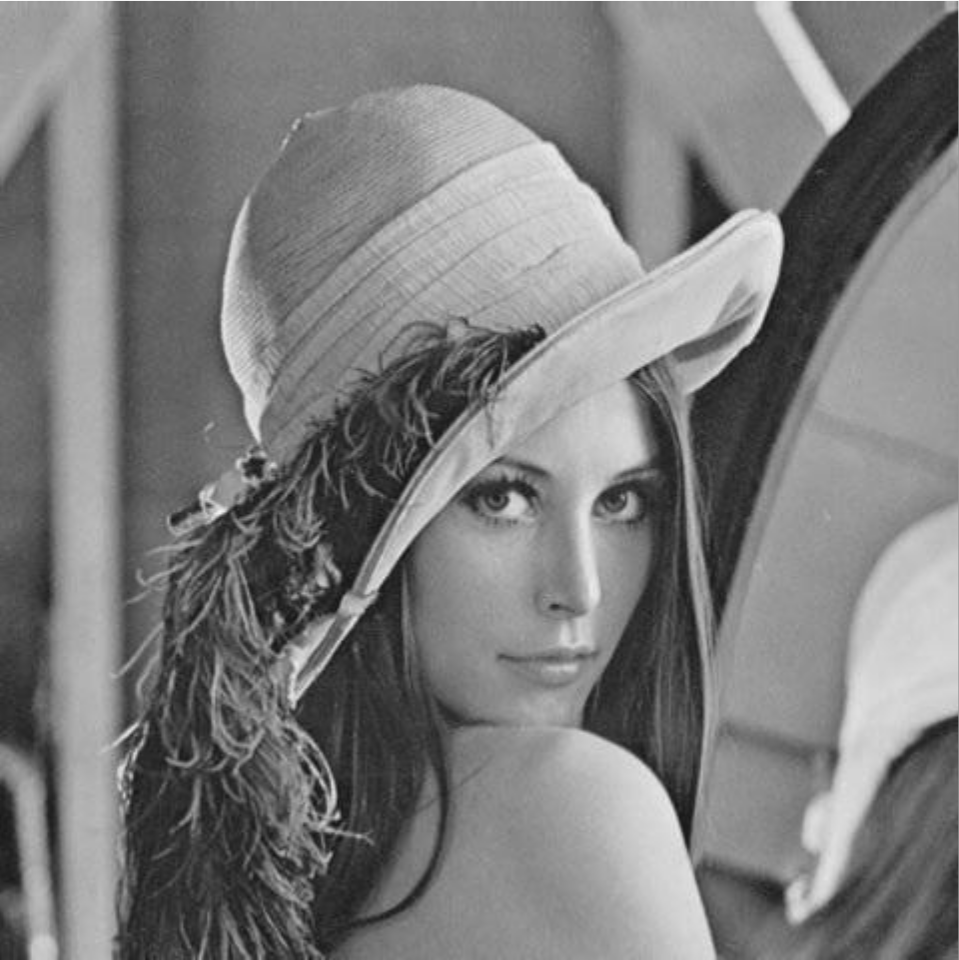
\includegraphics[height=200px]{canny-2.png}

Dieser Schritt ist notwendig, da der Algorithmus nur für die arbeit mit einem Farbkanal definiert ist.

\subsubsection*{(ii) Berechnung des Gradientenfeldes}

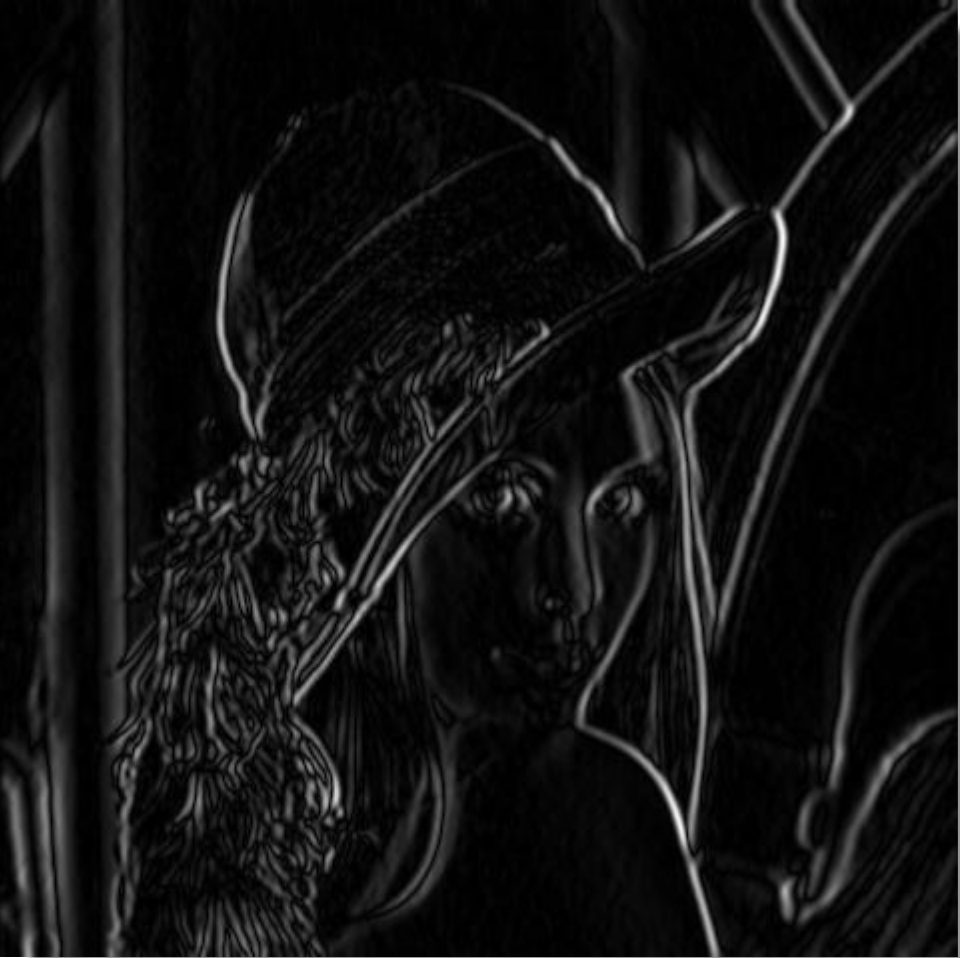
\includegraphics[height=200px]{canny-3.png}
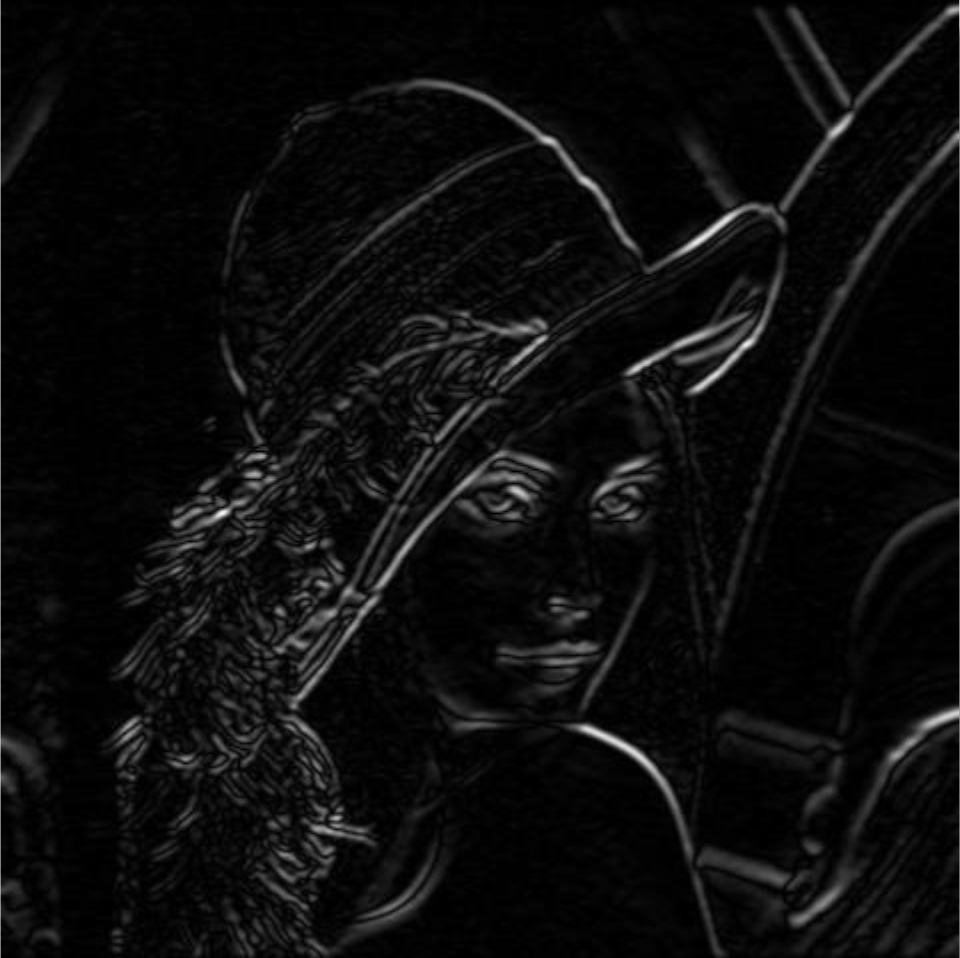
\includegraphics[height=200px]{canny-4.png}

Mit Gradientenfeld ist die Ableitung, also die Steigung (also somit das Gefälle -\textless Gradient) gemeint (siehe \hyperref[sec:difference-operator]{Differenzierungsoperator}). Wir berechnen diese Gradienten sowohl horizontal als auch vertikal und benutzen dafür konkret den \hyperref[sec:sobel-operator]{Sobel-Operator}

\subsubsection*{(iii) Bestimmung des Betrags der Gradientenvektoren}

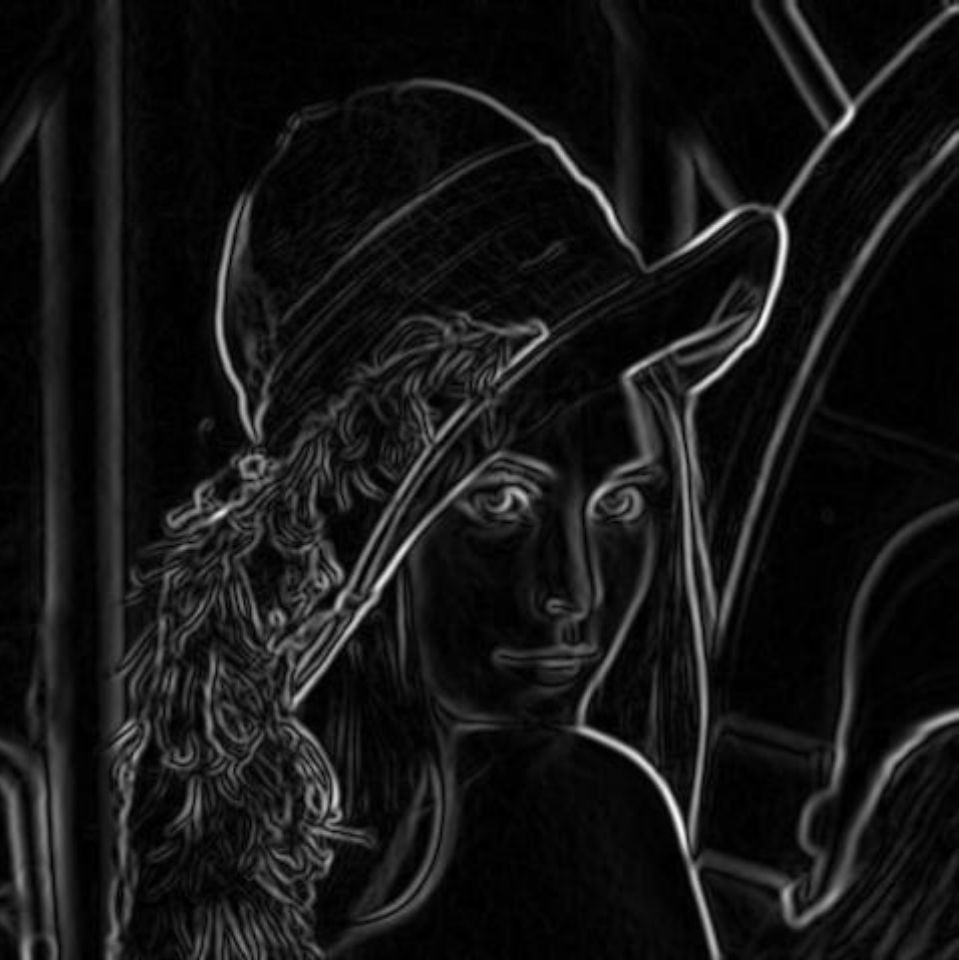
\includegraphics[height=200px]{canny-5.png}

Das Ziel dieses Schrittes ist es die vertikale und die horizontale Information zusammenzufügen. Dazu wird aus den beiden Werten für jedes Pixel ein 2-dimensionaler Vektor gebildet. Dann wird der Betrag (also die Länge) dieses Vektors berechnet. Das Ergebnis ist der neue Wert des Pixels.



\subsubsection*{(iv) Ausdünnen der Kanten - Non Maximum Suppression}

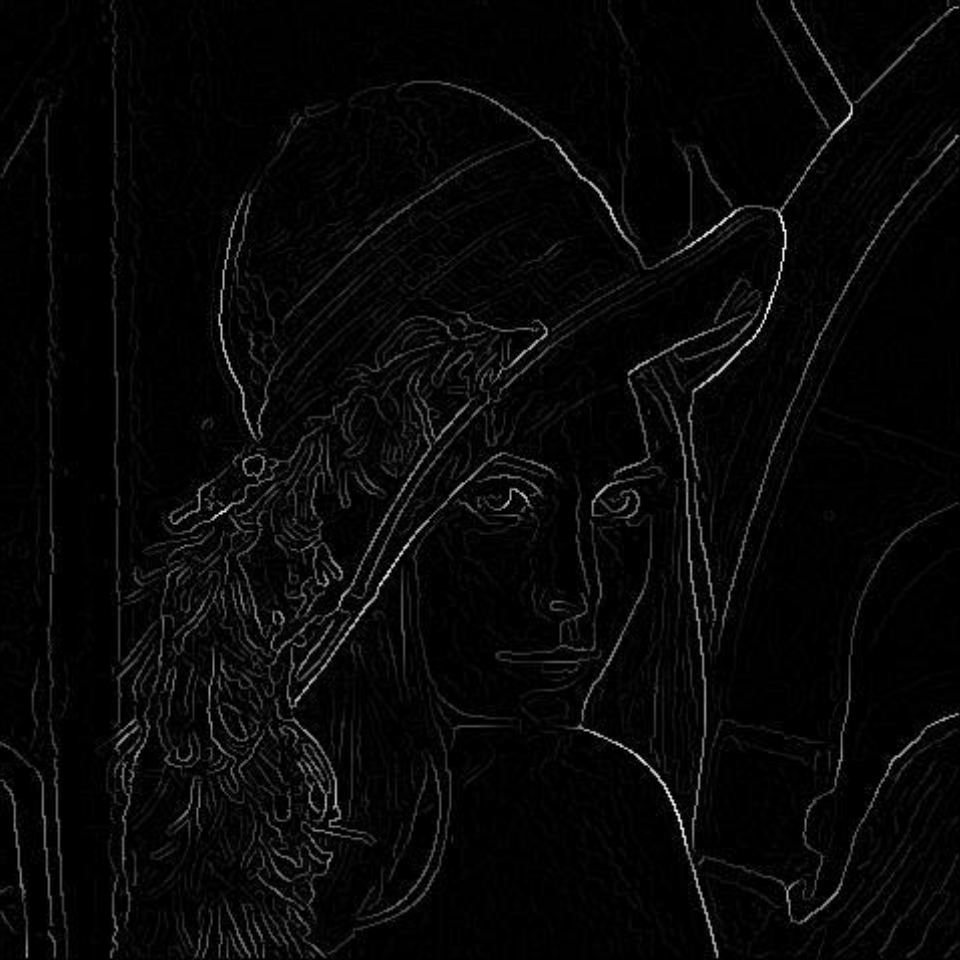
\includegraphics[height=200px]{canny-6.png}

Hiermit soll sichergestellt werden, dass jede Kante nur 1 pixel breit ist. Dazu wird eine 3x3-Matrix über das Bild verschoben, und jeweils alle Nicht-Maxima, d.h. alle 8 Werte außer dem größten Wert, auf 0 gesetzt.

\subsubsection*{(v) Hysterese}

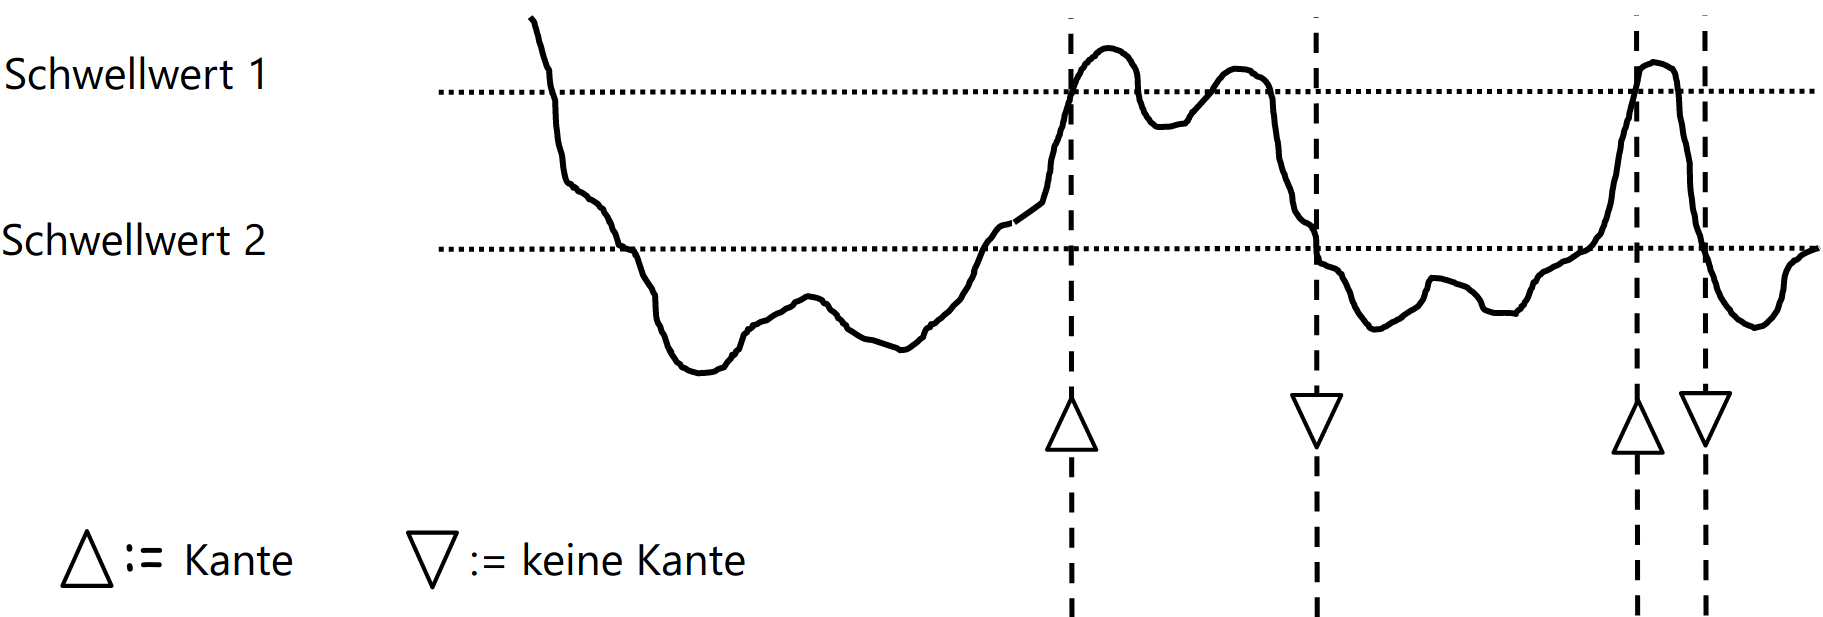
\includegraphics[height=150px]{canny-7.png}

Die Hysterese ist eine Art von \hyperref[sec:biniarisierung]{Biniarisierung}. Das heißt, dass wir mittels Schwellwerten einen Wert entweder behalten wollen (im Ergebnisbild weiß) oder entfernen wollen (im Ergebnisbild schwarz = Hintergrund). Im Gegensatz zur normalen Biniarisierung mit einem einzigen Schwellwert werden bei der Hysterese 2 Schwellwerte $ T_{1} < T_{2} $ verwendet.\\
Im ersten Schritt wird ein Pixel, wenn sein Wert größer als $T_{2}$ ist, als Bestandteil einer starken Kante eingestuft. Wenn ein Wert eines Pixels größer als $ T_{1} $ aber kleiner als $T_{2}$ ist, dann wird der Pixel als Bestandteil einer schwachen Kante eingestuft.\\
Im zweiten Schritt werden zunächst alle starken Kanten übernommen. Schwache Kanten werden nur dann übernommen, wenn sie starke Kanten berühren.\\

Das Ziel der Hysterese ist es nicht relevante schwache Kanten zu eliminieren. Im folgenden Ergebnisbild kann man sehen, dass z.B. die schwachen Kanten in der rechten unteren Ecke nicht übernommen wurden:

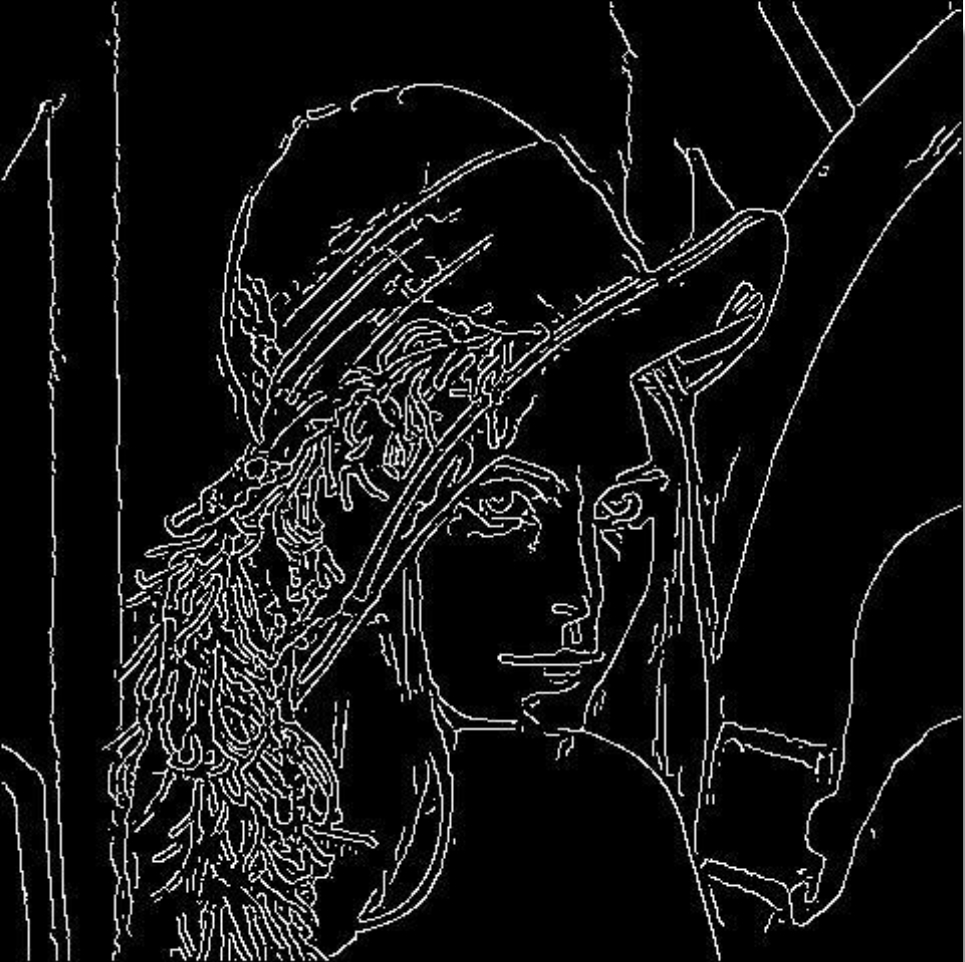
\includegraphics[height=200px]{canny-8.png}

\subsubsection{Hough-Transformation}

Die Hough-Transformation ist ein Verfahren zur Erkennung von Geraden, Kreisen oder anderen parametrisierbaren geometrischen Figuren in Bildern. Dabei ist schon bekannt welche Figur man erkennen möchte, man will aber die Position und Größe genau lokalisieren können. Wir wollen uns dies anhand von der Erkennung von Geraden ansehen.\\

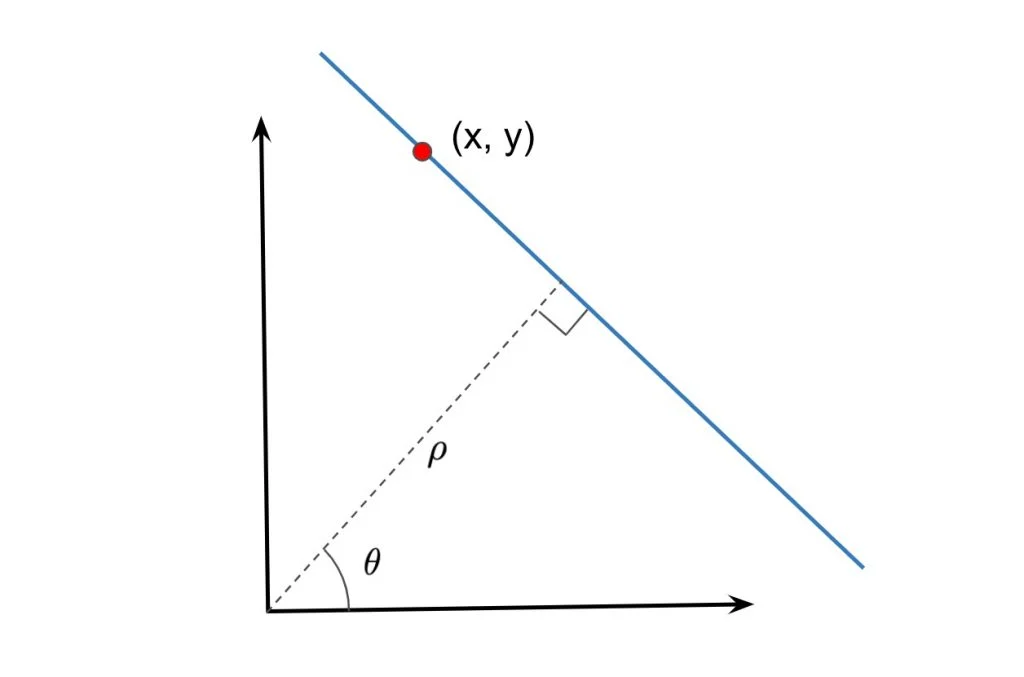
\includegraphics[height=200px]{hough-transformation-1.png}

Zunächst benötigen wir ein Eingangsbild, das die von uns zu erfassende Figur - die Gerade - möglichst eindeutig enthält. Um solch ein Bild aus einem realen Bild zu extrahieren können andere Algorithmen, wie z.B. der \hyperref[sec:canny-edge-detector]{Canny-Edge-Detector} verwendet werden.\\
Dann müssen wir festlegen mit welchen Parametern wir die Gerade darstellen wollen. Naheliegend wäre die Steigung und der y-Achsenabschnitt (klassische Darstellung linearer Funktionen). Doch hier entsteht das Problem, dass senkrechte Geraden nicht dargestellt werden können, da sie jedem x-Wert mehrere y-Werte zuordnen würde, also sozusagen eine ''unendliche Steigung'' hätte. Stattdessen können wir die Gerade auch mittels einem Winkel $\theta$ und einer Länge $p$ darstellen. Wir zeichnen eine Orthogonale zur Gerade, die durch den Ursprung verläuft. $\theta$ ist dann der Winkel der Orthogonalen zur x-Achse und $p$ die Länge dieser Orthogonalen. Der entstandene 2-dimensionale Vektorraum (im Grunde ein einfaches 2-dimensionales Koordinatensystem) wird auch Hough-Raum genannt. Jeder konkrete Punkt im Hough-Raum stellt also eine Gerade im Eingabebild dar.\\
Nun iterieren wir über alle relevanten Pixel des Eingangsbildes (die ja alle zu Kanten gehören, da das Bild entsprechend vorverarbeitet wurde) und finden errechnen für jeden Pixel alle möglichen Geraden, die diesen Punkt laufen. Mathematisch gesehen sind das natürlich unendlich viele Geraden, aber da unser Eingabebild nur begrenzt viele Pixel, also eine begrenzte Genauigkeit besitzt ist auch die Anzahl der verschiedenen Geraden im Bild endlich. Für jede dieser Geraden wird ein Wert, der dem entsprechende Punkt im Hough-Raum zugeordnet wird, inkrementiert. Es wird also sozusagen für diesen Punkt gevotet. Wir können die Werte, welche den Punkten im Hough-Raum zugeordnet werden dan mit Helligkeitswerten darstellen. Wenn wir das für alle Punkte durchgeführt haben, haben die Punkte im Hough-Raum, zu denen es am meisten Pixel im Eingangsbild gibt, die zu dieser Geraden gehören könnten, den höchsten Wert. Wenn man nun die Hochpunkte der Werte im Hough-Raum findet, so erhält man also die genauen Gleichungen für die Geraden im Bild und hat somit die Geraden identifiziert.

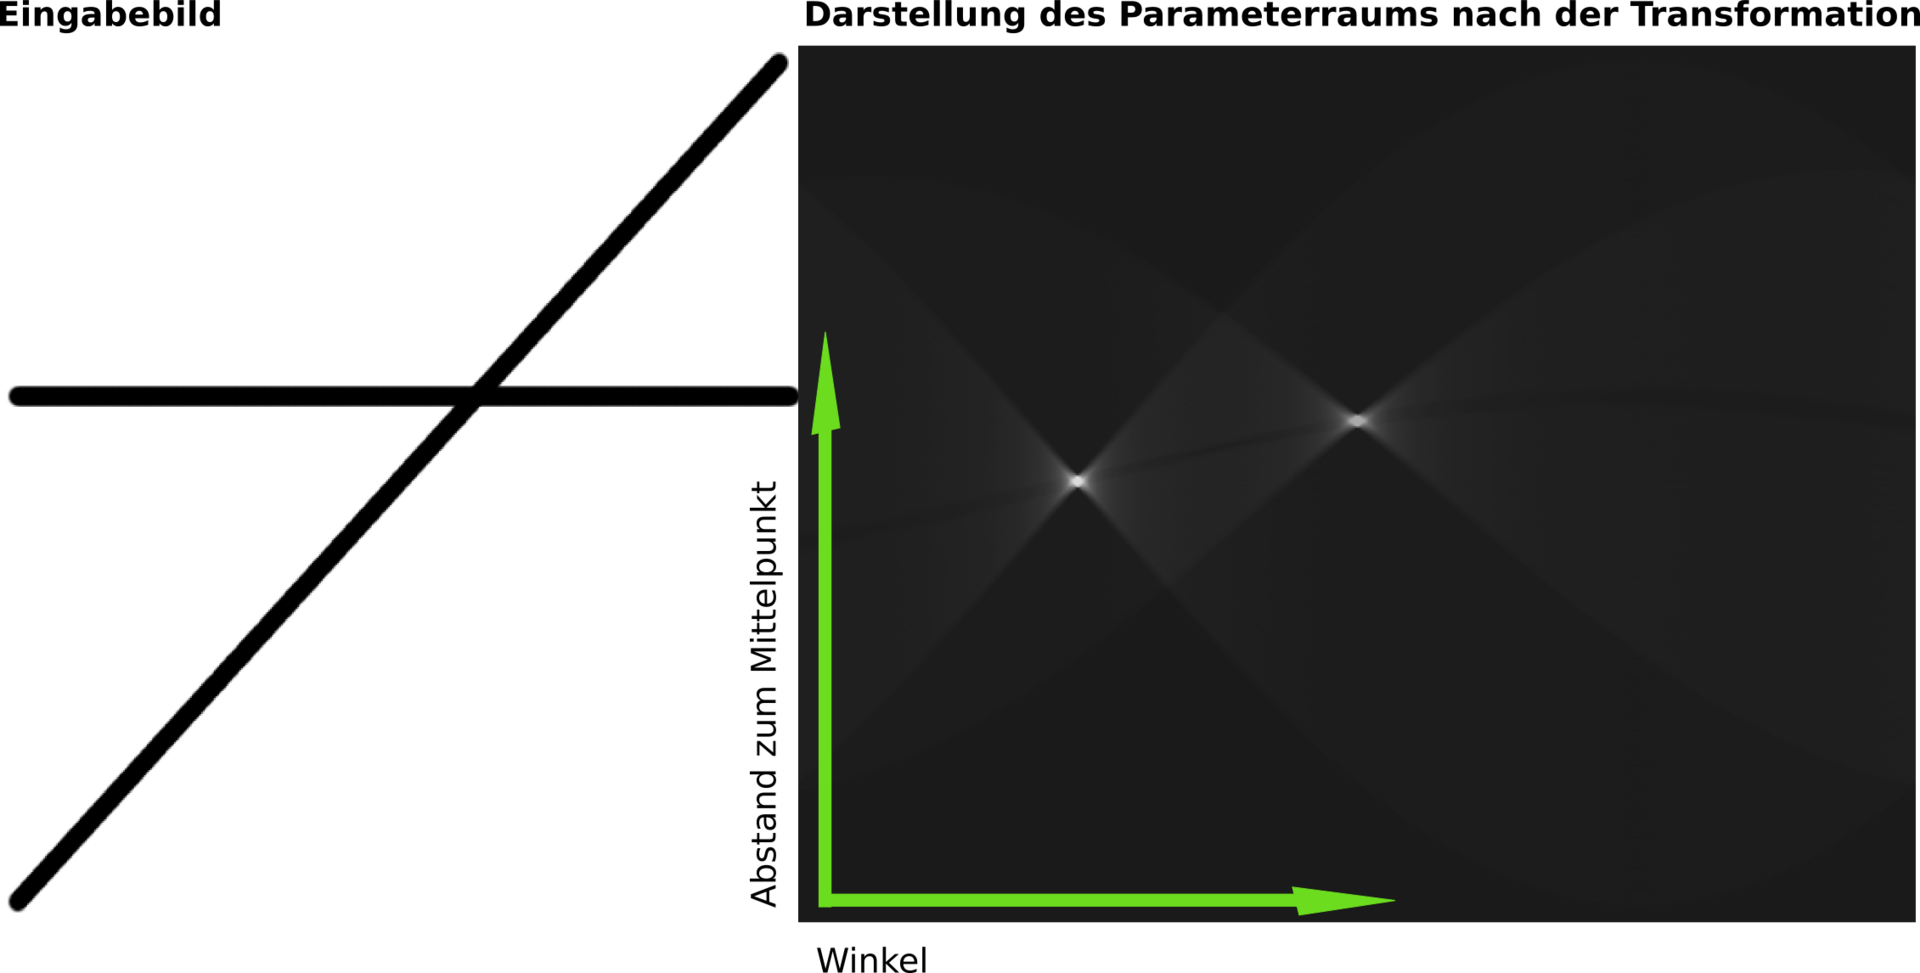
\includegraphics[height=200px]{hough-transformation-2.png}

\subsubsection{Harris-Corner-Edge-Detection}

Harris-Corner-Edge-Detection ist ein Verfahren zum Erkennen von Interest-Points. Interest-Points, oder auch Feature-Points genannt, sind Punkte, die man in verschiedenen Bildern der gleichen Szene oder des gleichen Objekts gut wiedererkennen kann. Die Erkennung von Interest-Points ermöglicht es z.B. automatisierte Objektverfolgung u.v.m. zu implementieren. Interest-Points sind also besonders signifikante Punkte, die möglichst aus verschiedenen Perspektiven trotzdem ähnlich aussehen.\\

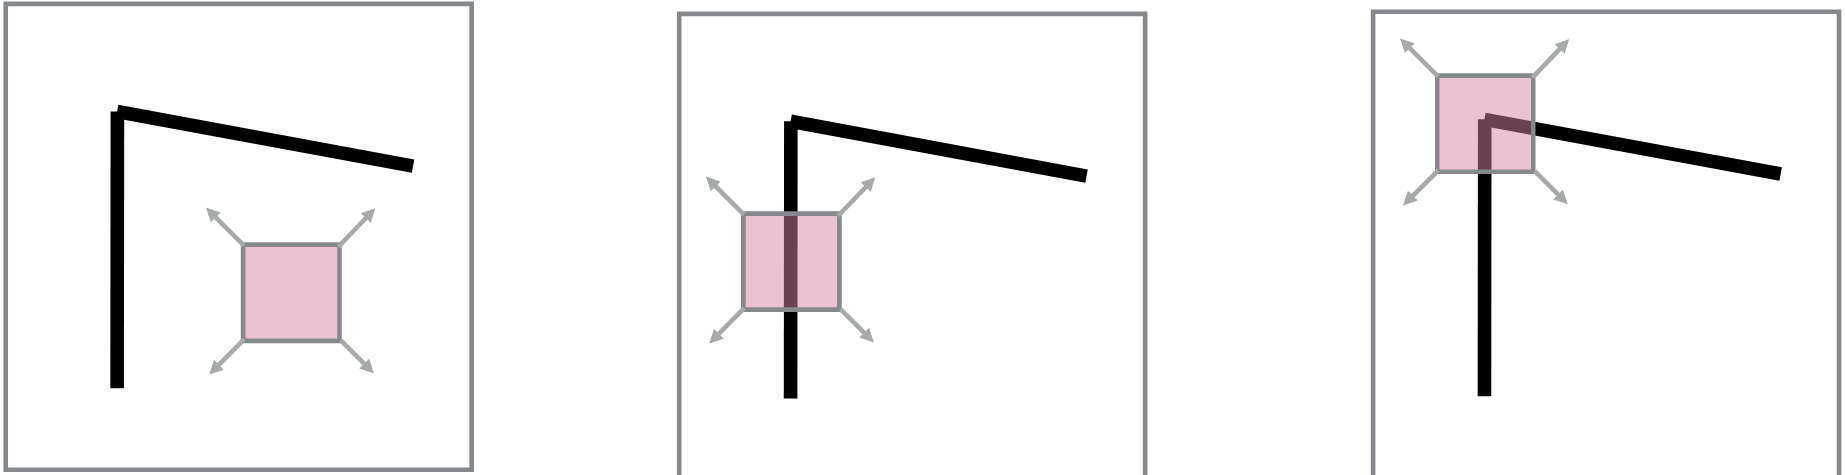
\includegraphics[height=125px]{harris-corner-edge.png}

Der Harris-Corner-Edge-Detector versucht signifikante Punkte zu finden, indem er misst wie verschieden ein Bereich von seinem Umfeld ist. Dabei wird gemessen wie groß der Unterschied der Pixelwerte ist, wenn man eine lokale-Nachbarschaftsmatrix um jeweils ein Pixel in jede Richtung verschiebt. Man erkennt im Beispiel:
\begin{itemize}
    \item \textbf{Im erstem Bild} verändern sich die Pixelwerte überhaupt nicht
    \item \textbf{Im zweiten Bild} verändern sich die Pixelwerte bei der vertikalen Verschiebung nicht
    \item \textbf{Im dritten Bild} verändern sich die Pixelwerte in jedem Fall $\rightarrow$ Iterest-Point gefunden
\end{itemize}

\subsubsection{SIFT - Scale-invariant Feature Transform}
\label{sec:sift}
SIFT ist ein Feature-Point-Detektionsalgorithmus, der eine lokale Umgebung auf eine Menge von Vektoren, sog. feature-vectors, abbildet. Das besondere der entstandenen feature-vectors ist, das sie so berechnet sind, dass sie weitestgehend unabhängig von Translation, Skalierung und Rotation des Objektes sind, das sie beschreiben. Dadurch ergeben sich für das gleiche Objekt aus einer anderen Perspektive die gleichen feature-vectors. Sucht man nur ein bestimmtes bekanntes Objekt in einem Bild, dann kann man es anhand seiner Menge an feature-vectors ermitteln. Auf die Details der Berechnung soll hier nicht näher eingegangen werden.

\subsubsection{Template Matching}

Wir haben bereits die Hough-Transformation kennengelernt, um Geometrische Formen in einem Bild zu erkennen, wie etwa Linien oder Kreise. Wenn wir aber komplexere Objekte erkennen möchten, die sich nicht einfach durch mathematische Zusammenhänge beschreiben lassen, müssen wir Template Matching betreiben. Der Input, den ein Template-Matching-Algorithmus verarbeitet sind ein Eingabebild, in dem gesuchte werden soll und ein Template, das angibt nach was gesucht werden soll. Der gewünschte Output ist dann die Position des gesuchten Objektes im Bild. \\

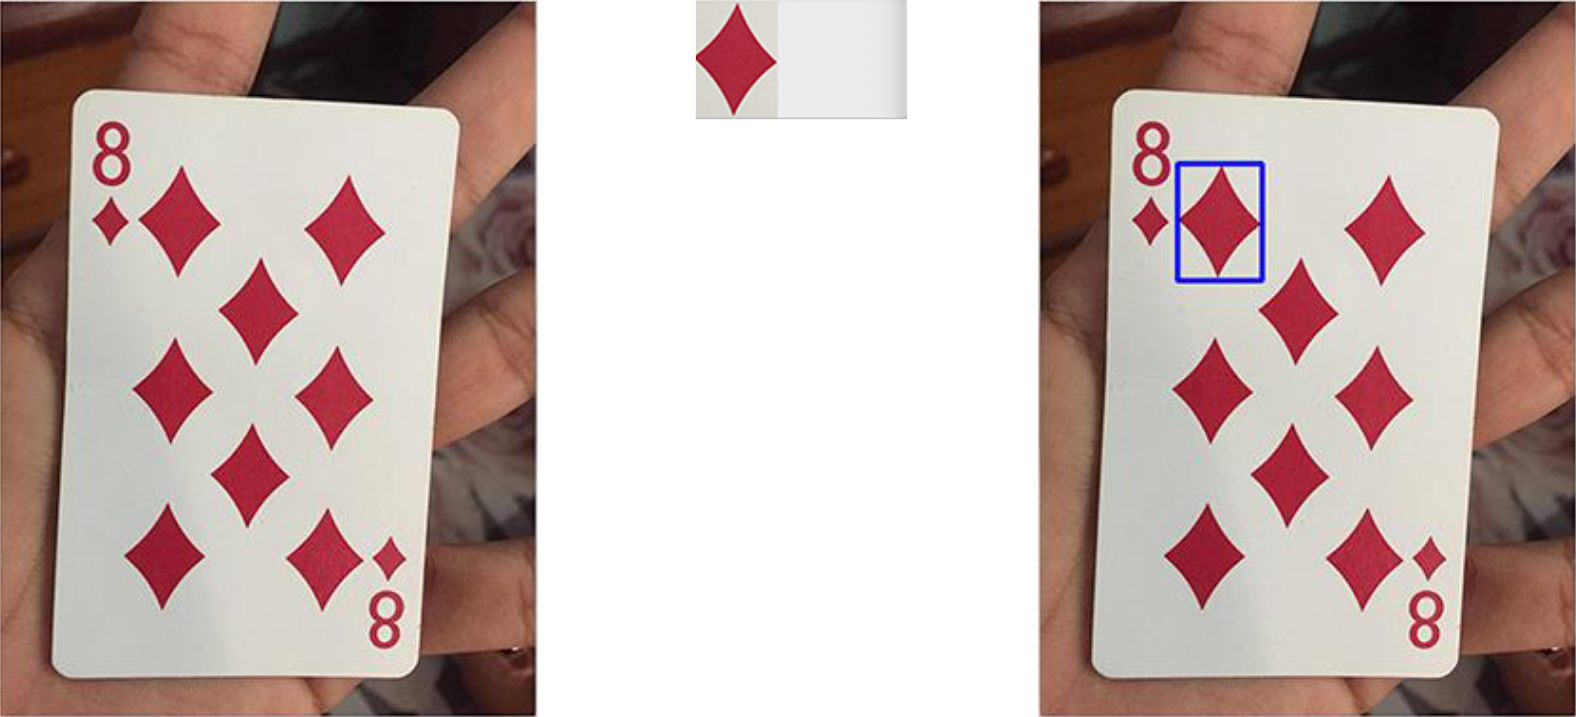
\includegraphics[height=150px]{TemplateMatching3.png}

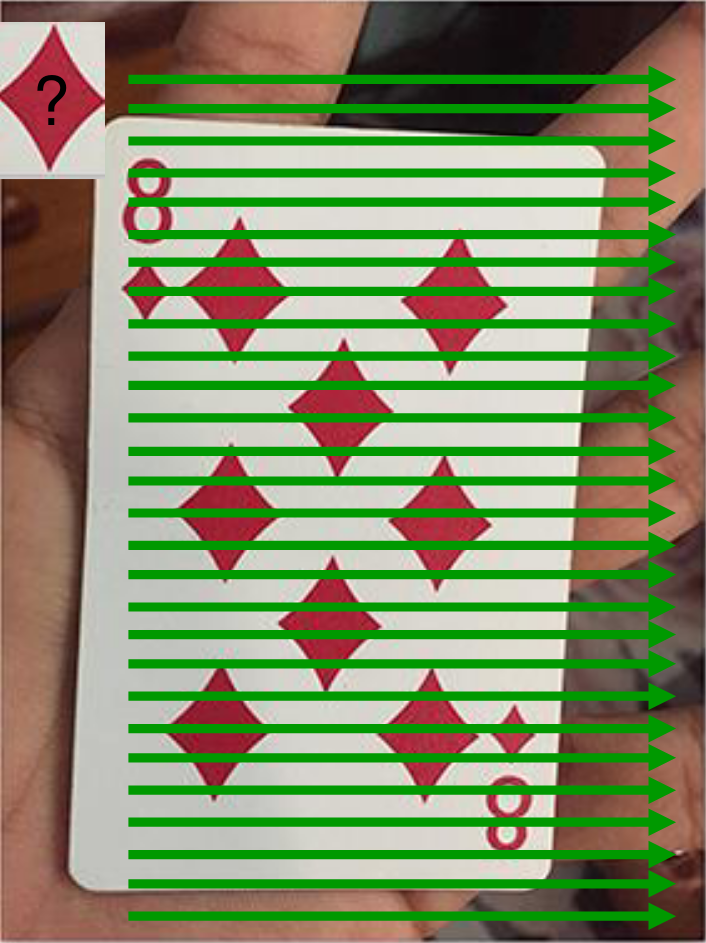
\includegraphics[height=150px]{templateMatching1.png}
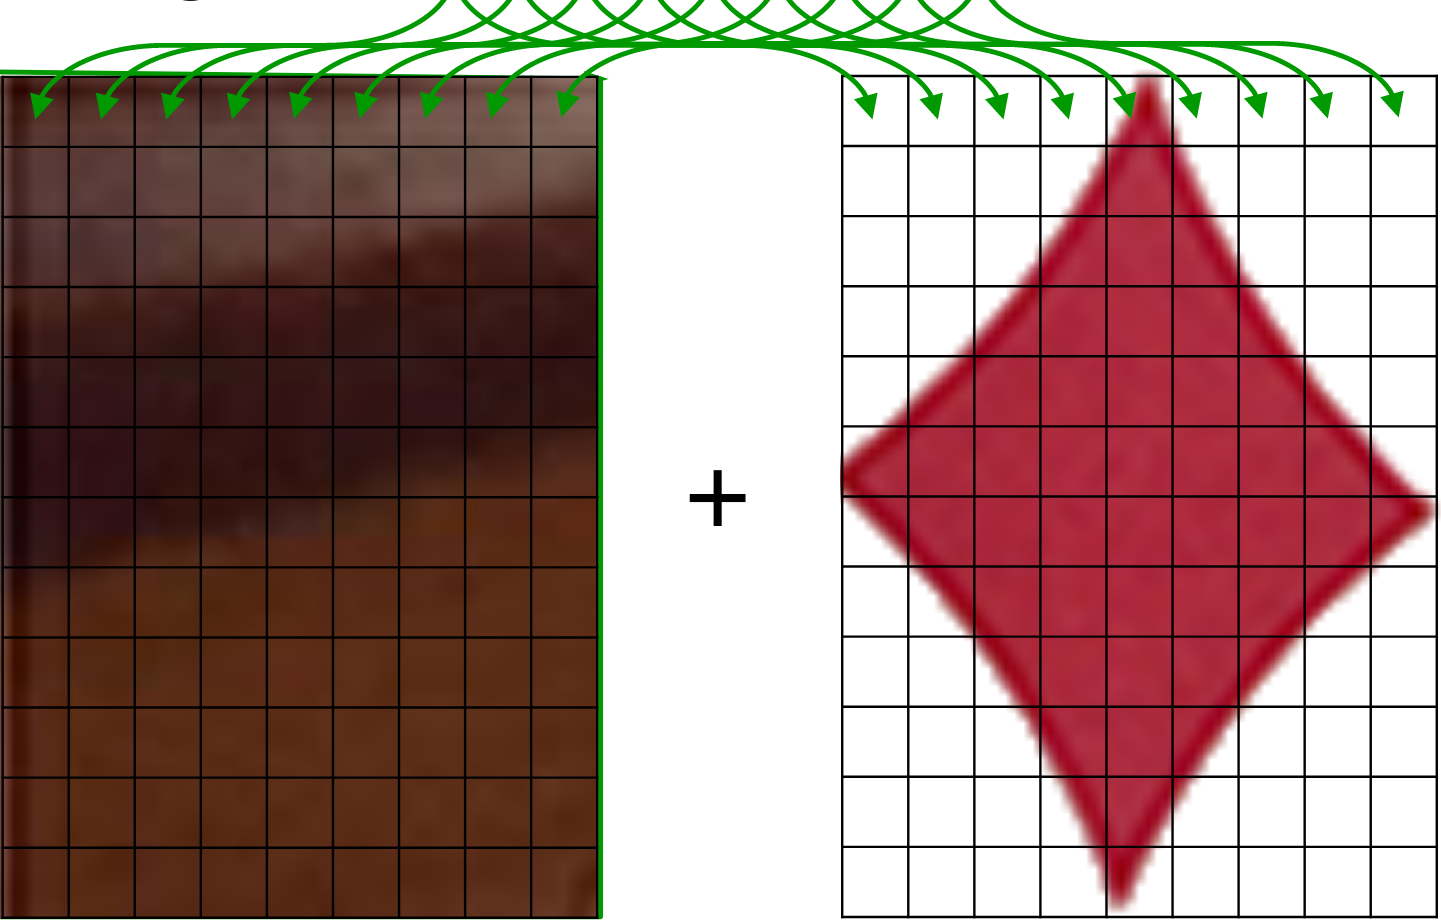
\includegraphics[height=150px]{TemplateMatching2.png}

Um das zu bewerkstelligen, kann für jede Möglichkeit das Template auf dem Eingabebild zu platzieren berechnet werden, wie hoch die Abweichung ist. Wenn der Fehler unter einem gewissen Schwellwert liegt, kann man festlegen, dass ein Match erkannt werden soll. Für die Berechnung des Fehlers kann z.B. der Betrag der Summe der pixelweisen Differenzen $F_{1}$ herangezogen werden, oder auch die Summe der Quadrate der pixelweisen Differenzen $F_{2}$:

\[
    F_{1} = \sum_{k=0}^{n}|P_{0}(x, y) - P_{1}(x, y)|
\]

\[
    F_{2} = \sum_{k=0}^{n}(P_{0}(x, y) - P_{1}(x, y))^{2}
\]

Die Schwierigkeiten beim Template Matching sind Abweichungen der Größe, Rotation, veränderte Belichtung und anderer Hintergrund des gesuchten Bereichs im Eingabebild. Es entstehen also insgesamt sehr viele Möglichkeiten, wie das Template im Bild versteckt werden kann. Im Gegensatz zum Brute-Force-Ansatz, bei dem wir alle Möglichkeiten durchprobieren würden, also etwa mit verschiedenen Drehwinkeln und Größen des Templates, gibt es auch noch den Ansatz mit Deep-Learning-Algorithmen. Bei diesem Ansatz berechnet der Algorithmus Feature-Vektoren, die im besten Fall weitestgehend invariant im Bezug auf verschiedene Transformationen, Clutter im Bild und veränderte Lichtverhältnisse sind.

\subsubsection{Image Stitching}

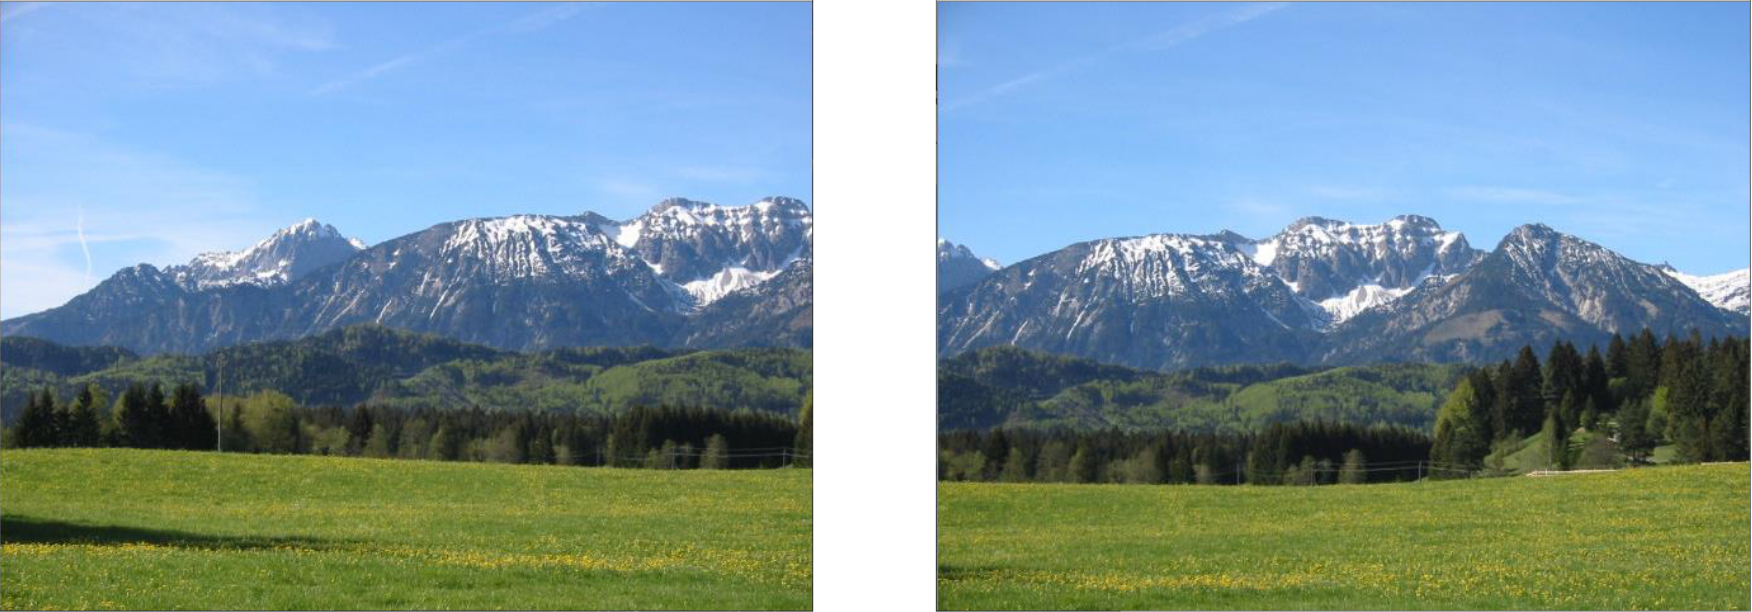
\includegraphics[height=150px]{imageStitching.png}

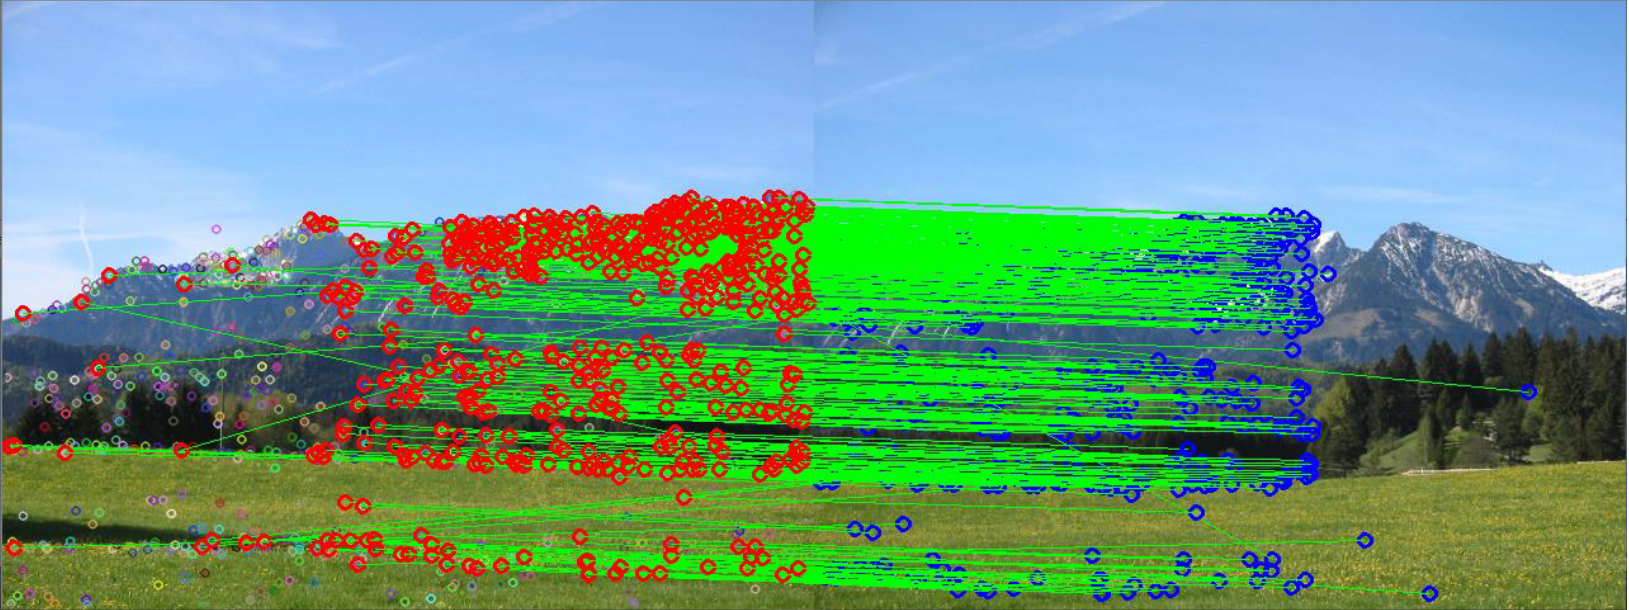
\includegraphics[height=150px]{featureMatches.png}

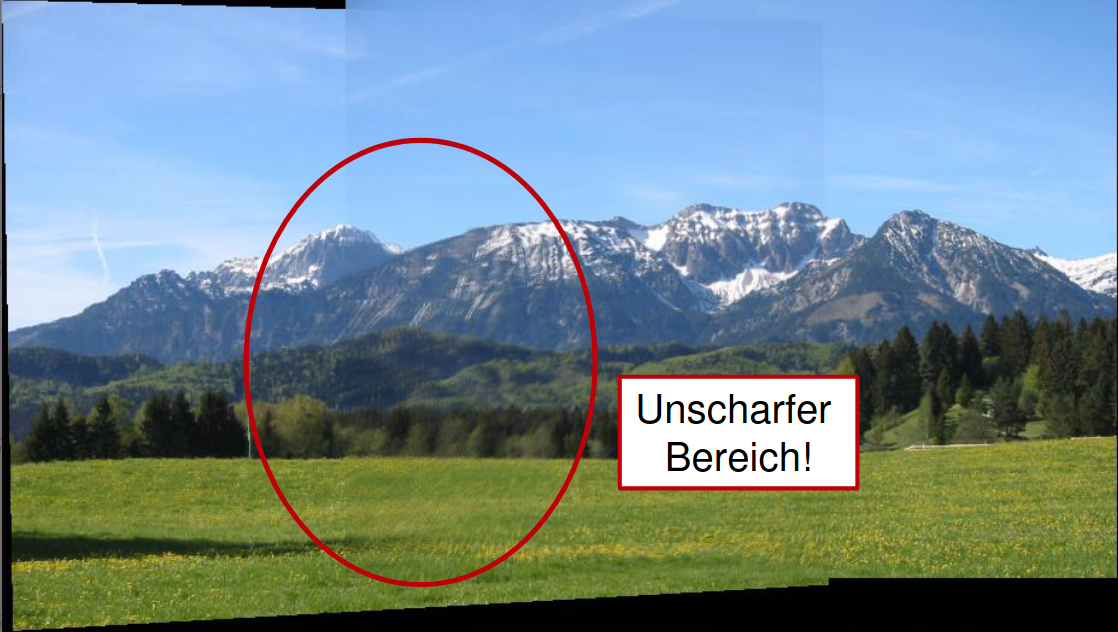
\includegraphics[height=150px]{panorama.png}

Beim Image Stitching geht es darum aus mehreren Teilbildern ein gemeinsames Bild zu erzeugen. Ein gutes Beispiel ist die Panorama-Funktion eines Handys, bei der man mehrere Bilder aufnimmt, die dann zusammengefügt werden. Die Grundlegende Herangehensweise ist die folgende:

\begin{enumerate}
    \item \textbf{Identifizieren von Feature Points:}\\
          Zunächst müssen Feature Points, also markante Punkte im Bild, erkannt werden. Hierfür kann z.B. der \hyperref[sec:sift]{SIFT-Algorithmus} verwendet werden
    \item \textbf{Finden von Feature-Pairs:}\\
          Dann müssen Feature-Pairs, also Paare aus Feature-Points der beiden Bildern, die zu den selben Objekten gehören, gefunden werden
    \item \textbf{Berechnung der Homografie:}\\
          Basierend auf den Vektoren, die die Feature-Pairs verbinden kann eine Homografie berechnet werden. Die Homografie ist das Verhältnis der beiden Kamerapositionen der beiden Bilder.
    \item \textbf{Zusamenfügen der Bilder:}\\
          Die Bilder werden an geeigneter Stelle übereinandergelegt
    \item \textbf{Morphing:}\\
          Wenn wir im überlappenden Bereich einfach die Mittelwerte der Pixelwerte bilden führt dies zu einer Unschärfe. Das liegt daran, dass die Bilder auf verschiedenen Winkeln geschossen sind und die Bereiche also nicht komplett identisch aussehen. Wir haben also 2 leicht verschiedene Bilder und wir wollen das Bild errechnen, dass sich im Übergang von einem Bild zum anderen Befindet. Den Prozess des findens dieses Übergansbildes nennt man Morphing.
\end{enumerate}